\documentclass[a4paper, 12pt, titlepage=true]{scrreprt}
\usepackage{graphicx,wrapfig}
\usepackage{subcaption}
\usepackage[ngerman]{varioref}
\usepackage[utf8]{inputenc}
\usepackage{harvard}
\usepackage[ngerman]{babel}
\usepackage[babel,german=swiss]{csquotes}
\usepackage[usenames,dvipsnames]{color}
%\usepackage{fancyhdr}
%\usepackage{rotating}
%\usepackage{multicol}
%\usepackage{floatflt}
\usepackage{enumerate}
%\usepackage{longtable}
%\usepackage{tikz}
%\usepackage{amsmath}
\usepackage[left=25mm,right=25mm,top=25mm,bottom=35mm]{geometry}
%\usepackage{enumerate}
%\usepackage{wrapfig}
%\usepackage{caption}
%\usepackage{gensymb}
\usepackage{subfig}
\usepackage{booktabs}

\usepackage[toc,page]{appendix} %vermutlich nicht gebraucht
\usepackage{lscape}
\usepackage{sidecap}
\usepackage{multicol} %nicht gebraucht
\usepackage{float}
\usepackage{amssymb,amsmath}
\DeclareGraphicsExtensions{.png, .jpg, .jpeg, .eps}
\graphicspath{{./images/}}
\setlength{\fboxrule}{4pt}
\setlength{\fboxsep}{20pt}

\definecolor{blau}{cmyk}{1,0,0.,0}
\newcounter{loesung}[chapter]
\newcounter{aufgabe}[chapter]
\renewcommand{\labelenumi}{\arabic{enumi}.}
\renewcommand{\labelenumii}{\arabic{enumi}.\arabic{enumii}}

\newcommand{\aufgabe}{\refstepcounter{aufgabe}
\textbf{\vspace{5pt} \\ Aufgabe \thechapter.\theaufgabe: }}

\newcommand{\loesung}{\refstepcounter{loesung}
\textbf{\vspace{5pt} \\ Loesung \thechapter.\theloesung: }}

\begin{document}

\iffalse
So erstellt man eine Grafik mit seitlicher Beschriftung:
\begin{SCfigure}[1][h]
 	\centering
	\includegraphics[scale = 0.3]{Gelderhaltung}	
	\caption{\textsf{text}}
	\label{fig:Discriminatorslope}
\end{SCfigure}
\fi


%\pagestyle{fancy}
%\thispagestyle{empty}

%\author{\includegraphics[width=0.6\textwidth]{Fadenpendel}}
\title{Physik für Baustatiker \\ HSLU, HS 2017}
\author{Skript von \\ \bf{Marco Gähler}}
\maketitle

\tableofcontents


%Das Skript kann an einigen Orten noch verbessert werden. In den ersten Kapiteln sollten noch ein paar Aufgaben hinzugefügt werden, das Kapitel zu den Drehbewegungen ist dafür recht lang. Allenfalls könnte man Impuls, Stösse und Leistung weglassen. Wobei der Impuls für die Drehbewegungen wiederum recht spannend ist...
%einige Grafiken und Aufgaben stammen aus dem powerpoint skript für Maschienenbauern, dort sollte man die Notationen (subscripte) noch anpassen.
\chapter*{Vorwort}

Dies ist das Skript zum Physik Teil der Vorlesung Baustatik. Es ist eine vierwöchige Wiederholung von Stoff, welcher eigentlich bereits bekannt sein, vermutlich aber mindestens wieder etwas aufgefrischt werden sollte. Die Vorlesung wird so zum ersten mal gehalten und kann natürlich noch verbessert werden. Verbesserungsvorschläge und Kommentare können an marco.gaehler@hslu.ch geschickt werden.
\vspace{0.5cm}

Buchempfehlungen:\\
-W. Demtröder, Experimentalphysik 1\\
-P. Tipler, Physik für Wissenschaftler und Ingenieure (ist sehr umfangreich)

\vspace{0.5cm}

Der zeitliche Ablauf der Vorlesung ist ungefähr wie folgt:
\begin{table}[h]
\begin{tabular}{ l l }
Tag 1: & Einführung, Einheiten und Kinematik\\ %dafür sollte mehr Zeit investiert werden. Wer das nicht kann, der versteht auch die Drehbewegungen nicht.
Tag 2: & Kräfte\\
Tag 3: & Kräfte\\ % Hier wurde mal noch der Impuls eingeführt. Ob das sinnvoll ist, weiss ich nicht. Evtl. sollte man ihn weglassen. Der Raketenantrieb war sicher zu viel des guten.
Tag 4: & Energie\\
Tag 5: & Energie\\ %Leistung könnte man auch weglassen.
Tag 6: & Drehmoment\\
Tag 7: & Trägheitsmoment\\
Tag 8: & Trägheitsmoment\\
\end{tabular}
%\caption{Eine Liste mit den wichtigsten Einheitenvorsätzen.}
\end{table}


\chapter{Einführung und Einheiten}

In der Physik geht es darum, die Umwelt möglichst exakt zu beschreiben. Sie wird entsprechend auch zu den exakten Wissenschaften gezählt. Diese haben alle gemeinsam, dass man sie mathematisch beschreiben kann. Die hat natürlich den Vorteil gegenüber anderen Wissenschaften, z. B. Recht oder Medizin, dass es viel weniger Unklarheiten gibt. Andererseits sind wir Menschen eher intuitiv und haben ein recht schlechtes Gefühl für exakte Rechnungen, Statistik, etc. Entsprechend ist Physik ein recht anspruchsvolles Fach, dafür werden wir aber mit genauen Resultaten belohnt.

Um die Natur zu beschreiben, brauchen wir nicht nur reine Zahlen, sondern auch noch Einheiten. Dazu wurden vor gut 200 Jahren verschiedene Grössen definiert. Die Wichtigsten davon sind die sogenannten SI-Grundeinheiten Meter, Sekunde und Kilogramm (nicht Gramm!!). Anhand von diesen 3 Einheiten werden wir alle weiteren Einheiten in dieser Vorlesung ableiten können. Auch bei den Einheiten gilt, was bereits im ersten Absatz geschrieben wurde: Meistens wissen Sie, welche Einheiten das Schlussresultat haben sollte, aber es ist natürlich besser, wenn man es genau ausrechnet. Dies möchten wir nun kurz mit ein paar einfachen Beispielen verdeutlichen.

%Das hier ist die neue Version
Zuerst eine kleine Widerholung der Mathematik. Formen Sie folgende Gleichungen um: %sollten evtl. noch weitere Beispiele hinzugefügt werden.
\begin{equation}
x = y \cdot z \rightarrow y = \dots
\end{equation}
\begin{equation}
2 \cdot a^2/b = 8 \rightarrow b = \dots
\end{equation}
Wir können natürlich auch mehrere Gleichungen kombinieren. a(c) bedeutet, dass a nur noch von c abhängen soll, sie sollen also b loswerden. %auch hier sollten vermutlich ein paar weitere einfache Aufgaben hinzugefügt werden
\begin{equation}
3\cdot a/b = c, b = a^2 \rightarrow a(c) = \dots
\end{equation}
\begin{equation}
10 \cdot y^2 \cdot z = x, y = 1000\cdot z, y(x) = \dots
\end{equation}
Soweit kennen Sie (hoffentlich) alles aus dem Mathematikunterricht. Wir können a, b, x, y etc. aber auch durch andere Ausdrücke ersetzen, z.B. Einheiten. 
\begin{equation}
1km = 1000m \rightarrow 0.4\cdot 1km = \dots
\end{equation}
\begin{equation}
1us = 10^{-6}s, 1ms = 10^{-3}s \rightarrow 35 \cdot 1ms = \dots us
\end{equation}
\begin{equation}
1Jahr = \dots Tage = \dots Stunden = \dots Minuten = \dots Sekunden
\end{equation}
\begin{equation}
1um = 10^{-6}s, \frac{2\cdot 1um}{1s} = \frac{\dots m}{Jahr}
\end{equation}

Wenn wir Einheiten benutzen, rechnen wir damit also genau gleich, wie wenn wir in der Mathematik eine Unbekannte haben.  %noch ein paar Begründungen dazu, wie wir mit Einheiten rechnen. Und ein paar Anmerkungen zu den Einheitenvorsätzen.

\iffalse %Alte Version, welche ich abändern würde
\begin{enumerate}
\item $5h = \dots s$
\item Zwetschgen kosten $5.-/kg$. Eine Zwetschge wiegt $100g$. Wie viel kostet eine Zwetschge?
\end{enumerate}

Diese Aufgaben konnten sie hoffentlich ohne grössere Probleme lösen. Andererseits haben das Resultat vermutlich nicht wirklich ausgerechnet, sonder eher Ihrer Intuition vertraut und es durch ''konzentrisch hinsehen'' gefunden. Versuchen wir es mal mit etwas komplizierteren Rechnungen:

\begin{enumerate}
\item $3m^3 = \dots cm^3$
\item $3.6km/h = \dots m/s$
\item $20g/s = \dots kg/h$
\item Aprikosen kosten $7.20.-/kg$. Eine Aprikose wiegt $130g$. Wie viel kostet eine Aprikose?
\end{enumerate}

Schwierig? Jein. Ihre Intuition reicht hier nicht mehr aus, um diese Aufgaben zu lösen. Wenn man die Aufgabe aber systematisch angeht, kann man sie sehr schnell lösen. Schauen wir uns mal die erste Aufgabe an: $3m^3 = \dots cm^3$. Wir müssen also Kubikmeter in Kubikzentimeter umrechnen. Wir alle wissen, dass ein Meter genau 100 Zentimeter sind, also $1m = 100cm$. Aber wie soll man nun die Kubikmeter umrechnen? Wir setzen dies einfach in die obige Rechnung ein:
\begin{equation}
3m^3 = 3\cdot (1m)^3 = 3\cdot (100cm)^3 = 3\cdot 10^6 cm^3.
\end{equation}
Dass wir dabei noch den $m$ zu $1m$ umformen ist eigentlich nicht nötig, einen Schritt schneller ist noch
\begin{equation}
3m^3 = 3\cdot (100cm)^3 = 3\cdot 10^6 cm^3.
\end{equation}
Wir haben also in der Rechnung einfach $m = 100cm$ eingesetzt und damit gerechnet.

Das zweite Beispiel ist sehr bekannt. Der Tacho im Auto zeigt die Geschwindigkeit in $km/h$ an, die SI-Einheit ist aber $m/s$. Folglich muss man die beiden Grössen umformen. Wenn man nun wiederum verwendet, dass $km = 1000m$ und $h = 60min = 3600s$, ist die Umformung schnell gelöst:
\begin{equation}
3.6\frac{km}{h} = 3.6 \frac{1000m}{3600s} = 1\frac{m}{s}
\end{equation}

Genau gleich funktioniert es natürlich, wenn wir von kleinen zu Grossen Einheiten wechseln. $1kg = 1000g$ und $1g = \frac{1}{1000}kg$, sowie $1s = \frac{1}{3600}h$.
\begin{equation}
20\frac{g}{s} = 20\frac{\frac{1}{1000}kg}{\frac{1}{3600}h} = 20\frac{3600kg}{1000h} = 72kg/h.
\end{equation}
Hier muss man allerdings mit den Brüchen aufpassen, dass einem keine Fehler unterlaufen.

Zuletzt noch
\begin{equation}
\frac{Preis}{Stueck} = \frac{Preis}{Gewicht}\cdot \frac{Gewicht}{Stueck} = 7.20\frac{Fr.-}{kg}\cdot \frac{0.13kg}{1 Stueck} = 0.936Fr.- pro\; Stueck
\end{equation}

Man kann auch anhand der Einheiten raten, wie man die verschiedenen Grössen kombinieren muss, um das gewünschte Resultat erhalten. Beim letzten Beispiel suchen wir etwas mit den Einheiten $\frac{Fr.-}{Stueck}$ und haben Grössen mit den Einheiten $\frac{Fr.-}{kg}$, sowie $\frac{kg}{Stueck}$ gegeben. Entsprechend kann man auch einfach raten und die beiden Grössen miteinander multiplizieren, da $\frac{Fr.-}{Stueck} = \frac{Fr.-}{kg}\frac{kg}{Stueck}$ gilt. Ob man dabei einen Faktor $\pi$ falsch liegt, weiss man nicht, aber zumindest hat man gut geraten.

Versuchen Sie bei möglichst allen Aufgaben in dieser Vorlesung mit den Einheiten zu rechnen, und nicht nur die Zahlen hinzuschreiben. Dies ist eine gute Übung, und sie können so teilweise auch Fehler frühzeitig erkennen, falls die erhaltene Einheit nicht mit dem gesuchten Resultat übereinstimmt. 

\fi

\begin{table}[h]
\centering
\begin{tabular}{ c c c }
 Einheitenvorsatz & Abkürzung & Wert \\
 Tera & T & $10^{12}$ \\
 Giga & G & $10^9$\\
 Mega & M & $10^6$\\
 Kilo & k & $10^3$\\
 Hekto & h & $100$\\
 Dezi & d & $0.1$\\
 Zenti & c & $0.01$\\
 Milli  & m & $10^{-3}$\\
 Mirko & $\mu$ & $10^{-6}$\\
 Nano & n & $10^{-9}$\\
\end{tabular}
\caption{\textsf{Eine Liste mit den wichtigsten Einheitenvorsätzen.}}
\end{table}

%\section*{Aufgaben}
\aufgabe
Formen sie die folgenden Grössen um:
\begin{enumerate}[a)]
\item $350ms = \dots s$
\item $35ng = \dots mg$
\item $8m/s = \dots km/h$
\item $10\frac{kg}{dm^3} = \dots \frac{g}{cm^3}$
\item $\frac{5m}{(3s)^2} = \dots \frac{km}{h^2}$

\end{enumerate}

\chapter{Kinematik}
\section{Geschwindigkeit}
%Zuerst sollte man den Studenten evtl. die Aufgabe zum Stein geben, welcher man in den Brunnen wirft, um die Tiefe zu bestimmen. Wer diese Aufgabe lösen kann, darf gehen. Die Andern haben noch etwas zu tun.
%Wie meistens: Die Unterlagen sollten nochmals etwas überarbeitet werden...
Die Kinematik ist eine Grundlegende, und auch eine der einfachsten Theorien der Physik. Sie beschreibt die Bewegung von Körpern. Zuerst müssen wir dazu ein Koordinatensystem, sowie eine Zeit definieren. Wie wir das genau machen, ist uns überlassen. Am einfachsten wählen wir einfach mal bei Luzern den Ort $0km$ und starten eine Stoppuhr, wenn wir losfahren, $0:00:00$. Alle Distanzen und Zeiten werden von hier aus gemessen. Ein Auto fährt nun mit einer konstanten Geschwindigkeit von $100km/h$ in Richtung Zürich ($50km$ entfernt). Die ganze Fahrt dauert entsprechend $30min$. Wo befindet sich das Auto nach $12min$?
%Grafik zum Auto einfügen
\begin{figure}[h]
 	\centering
	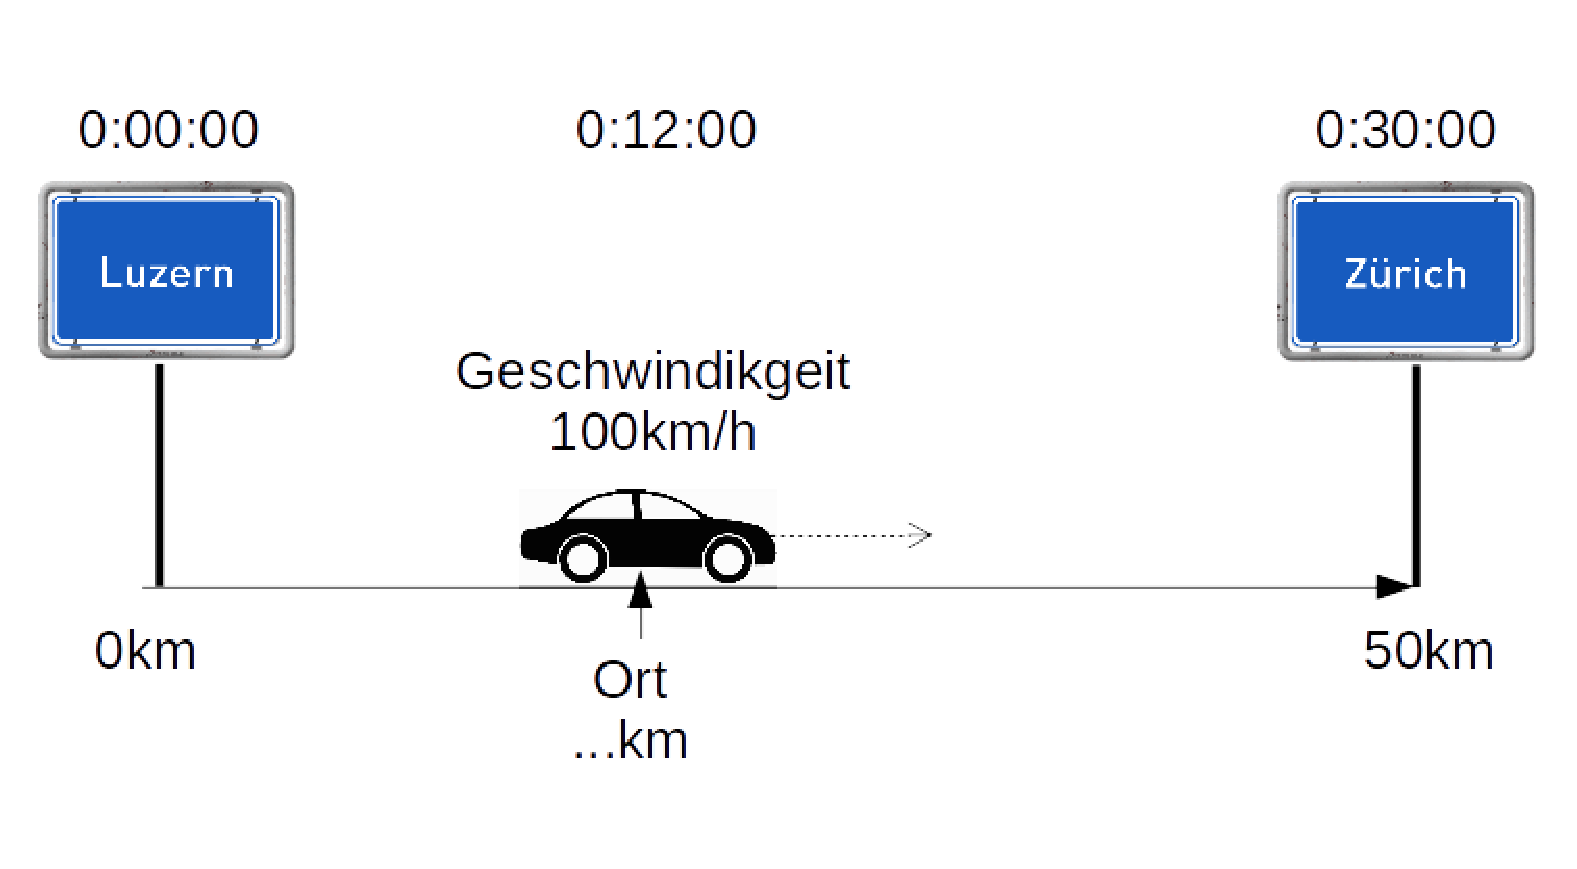
\includegraphics[scale = 0.6]{Kinematik_Auto2}	
	\caption{\textsf{text}}
	\label{fig:Discriminatorslope}
\end{figure}

Diese Aufgabe haben zumindest ein paar von Ihnen ähnlich gelöst, wie im vorhergehenden Kapitel: Mit einem Dreisatz. $12min$ ist Zwei Fünftel von $30min$, folglich befindet sich das Auto an Zwei Fünftel von $50km$, also bei $20km$. Das ist natürlich richtig, aber wir wollen diese ganzen Rechnungen nun auf ein etwas solideres Fundament stellen. Bisher haben wir ja erst den Ort und die Zeit definiert. Dabei konnten wir jeweils den Nullpunkt selber wählen, und messen die Distanzen von dort aus mit einem sehr langen Meter und einer Stoppuhr. Die Durchschnittsgeschwindigkeit definieren wir nun mathematisch als 
\begin{equation}
Durchschnittsgeschwindigkeit = \frac{zurueckgelegte\; Strecke}{benoetigte\; Zeit}.
\end{equation}
Da man in der Physik aber sehr viele solcher Formeln schreibt, möchte man diese Gleichung in eine etwas kürzere Form bringen. Dafür wurden die Formelzeichen eingeführt. Dies sind Abkürzungen für die oben geschriebenen Grössen, welche aus einem einzelnen Buchstaben bestehen. Für die oben verwendeten Grössen sind dies:
\begin{itemize}
\item Durchschnittsgeschwindigkeit $= \overline{v}$
\item Strecke, Ort $= s$
\item Zeit $= t$
\end{itemize}
Dabei muss man natürlich aufpassen, dass die Formelzeichen eindeutig sind. Wenn man zum Beispiel ein rotes und ein blaues Auto hat, kann man die Geschwindigkeiten unterscheiden, indem man diese als $\overline{v}_{rot}$ und $\overline{v}_{blau}$ bezeichnet, indem man die Autos nummeriert, oder sonst irgendwie kennzeichnet. Wichtig ist einfach, dass die aufgeschriebene Rechnung eindeutig ist, und man sie versteht. Teilweise wird die Durchschnittsgeschwindigkeit auch als $v$ ohne Strich darüber geschrieben. Unsere Schreibweise hier hat aber den Vorteil, dass wir nicht die Geschwindigkeit und die Durchschnittsgeschwindigkeit verwechseln. Schreiben wir die oben erwähnte Gleichung mal mit den Formelzeichen hin:
\begin{equation}
\overline{v} = \frac{s}{t}
\end{equation}
Damit können wir nun auch rechnen, wie Sie es aus dem Mathematikunterricht kennen. Wenn wir wissen möchten, wie weit das Auto in $12min$ gefahren ist, müssen wir die Gleichung nach dem Ort $s$ auflösen. Dazu multiplizieren wir beidseitig mit der Zeit $t$ und erhalten
\begin{equation}
s = \overline{v}\cdot t.
\label{eq:Ort1}
\end{equation}
Nun können wir die erwähnten Werte einsetzen und erhalten ebenfalls unser Resultat:
\begin{equation}
s = \overline{v}\cdot t = 100km/h \cdot 12min = 100km/h\cdot 12\frac{h}{60} = 20km.
\end{equation}
Dabei haben wir wiederum verwendet, dass eine Minute einen Sechzigstel einer Stunde ist, also $min = \frac{h}{60}$.

\section{Beschleunigung}
Etwas komplizierter wird die Sache, wenn die Geschwindigkeit nicht mehr konstant ist. Nun gibt es neben der Durchschnittsgeschwindigkeit auch noch die Grösse der Momentangeschwindigkeit. Die Momentangeschwindigkeit ist das, was der Tachometer im Auto anzeigt. Dabei wird immer in ganz kurzen Zeitabständen $\Delta t$ gemessen, welche (kurze) Distanz $\Delta s$ zurückgelegt wurde. Kurz ist dabei natürlich relativ zur Zeit, welche man für die Beschleunigung braucht. Bei einem Auto z.B. eine Sekunde. Die Momentangeschwindigkeit $v$ ist dann definiert als
\begin{equation}
Momentangeschwindigkeit = \frac{kurze\; Strecke}{kurze\; Zeiteinheit} = \frac{\Delta s}{\Delta t} = \frac{ds}{dt}.
\end{equation}
Die letzte Schreibweise ist die zeitliche Ableitung des Ortes nach der Zeit und die genaue Definition der Geschwindigkeit. Darauf werden wir hier aber nicht weiter darauf eingehen.

Die Beschleunigung $a$ beschreibt die Geschwindigkeitsänderung $\Delta v$ pro Zeiteinheit $\Delta t$, also
\begin{equation}
a = \frac{\Delta v}{\Delta t}.
\end{equation}
Die Einheit von $[a]$ beträgt 
\begin{equation}
[a] = \frac{[v]}{[t]} = \frac{m/s}{s} = \frac{m}{s^2}.
\end{equation}
Die Einheit ist einfach so wegen den Regeln der Mathematik. Dabei am besten verliert man darüber keine grosse Gedanken und versuchen Sie ja nicht, sich die Quadratsekunden irgendwie vorzustellen! Der Wert $a = 5m/s^2$ besagt einfach, dass die Geschwindigkeit pro Sekunde um $5m/s$ zunimmt.

Die Geschwindigkeitsänderung während einer konstanten Beschleunigung gegeben durch
\begin{equation}
\Delta v = a\cdot \Delta t.
\end{equation}
Die Geschwindigkeit nach der Beschleunigung hängt natürlich auch noch von der Geschwindigkeit vor der Beschleunigung ab. Mit der obigen Formel haben wir ja nur die Veränderung ausgerechnet. Die gesamte Formel um die Geschwindigkeit auszurechnen ist gegeben durch
\begin{equation}
v = v_0 + \Delta v = v_0 + a\cdot \Delta t,
\end{equation}
Wobei $v_0$ die Anfangsgeschwindigkeit ist. Bei einer Anfangsgeschwindigkeit $v_0$ und einer konstanten Beschleunigung $a$ ist die Momentangeschwindigkeit $v$ also gegeben durch
\begin{equation}
v(t) = v_0 + a\cdot t.
\end{equation}

Um die während einer Zeit $t$ zurückgelegte Strecke zu berechnen, müssen wir nun noch bestimmen, wie die Durchschnittsgeschwindigkeit und die Momentangeschwindigkeit zusammenhängen. Wir betrachten wiederum nur den Fall für eine konstante Beschleunigung. Da die Geschwindigkeit dabei linear zunimmt, ist die Durchschnittsgeschwindigkeit genau der Durchschnitt aus der Anfangs- und der Endgeschwindigkeit, also
%Grafik für den Durchschnitt
\begin{equation}
\overline{v} = \frac{v_0 + (v_0+a\cdot t)}{2} = v_0 + \frac{a\cdot t}{2}.
\end{equation}
Dies setzen wir nun in die Gleichung \ref{eq:Ort1} ein und erhalten
\begin{equation}
s = v_0\cdot t + \frac{1}{2}a\cdot t^2.
\end{equation}
Wenn man den Anfangsort $s_0$ nicht bei 0 gewählt hat, muss man diesen natürlich auch noch in die Gleichung einfügen,
\begin{equation}
s = s_0 + v_0\cdot t + \frac{1}{2}a\cdot t^2.
\end{equation}

%grafische Darstellung von Bewegungen?

\section{Gravitationsbeschleunigung}
Wenn Ihnen Ihr iPhone aus der Hand fällt, hat dieses zu Beginn des Falles noch keine Vertikalgeschwindigkeit. Am Boden ist es aber schon ziemlich schnell und wird entsprechend beschädigt. Es hat also in kurzer Zeit an Geschwindigkeit gewonnen. Die entsprechende Beschleunigung ist für alle Widerstandsfreien Körper (ohne Luftwiderstand) und überall auf unserem Planeten etwa gleich gross. Sie beträgt $g = 9.81m/s^2$ und wird Gravitationsbeschleunigung genannt. Für Körper im Freien Fall können wir auch mit den bereits behandelten Formeln rechnen, wobei wir nun natürlich Bewegungen in der Vertikalen betrachten und die Beschleunigung immer jeweils durch $a = g$ gegeben ist.

\aufgabe Sie fahren mit dem Fahrrad über einen Berg. Auf dem 5km langen Aufstieg fahren Sie mit $15km/h$, auf der $20km$ langen Abfahrt mit $40km/h$. Wie lange brauchen Sie für die gesamte Fahrt?

\aufgabe Sie fahren mit dem Auto nach Olten (60km Distanz). Sie haben dafür 1 Stunde eingeplant. Die erste Hälfte der Strecke können Sie aber nur mit $40km/h$ fahren. Wie schnell müssen sie auf der restlichen Strecke fahren? 

\aufgabe Sie stehen oben an einer überhängenden Felswand und lassen einen Stein fallen. Nach 2 Sekunden schlägt er auf dem Boden auf. Wie hoch ist die Felswand?

\aufgabe Max und Anna machen ein Rennen. Da Anna aber schneller ist (sie $8m/s$, er $7m/s$), erhält Max 10 Meter Vorsprung. Ab welcher Distanz gewinnt Anna das Rennen?

\aufgabe Sie fahren mit $50km/h$. Sie beschleunigen $3s$ lang mit $2m/s^2$. Wie schnell sind sie nachher?

\aufgabe Sie beschleunigen $4s$ lang mit $2m/s^2$. Nachher haben Sie eine Geschwindigkeit von $15m/s$. Wie schnell waren sie vor der Beschleunigungsphase?

\aufgabe Sie rennen mit $5m/s$ an einem stehenden Motorrad vorbei. Genau in diesem Augenblick beginnt es mit $2m/s^2$ zu beschleunigen. Nach wie viel Zeit werden Sie wieder überholt?

\aufgabe Sie lassen wiederum einen Stein von einer Felswand fallen. Nach $4s$ hören Sie den Aufschlag. Wie hoch ist die Felswand, wenn die Schallgeschwindigkeit $330m/s$ beträgt? (Die entstehende quadratische Gleichung muss nicht gelöst werden, da dies von Hand SEHR mühsam wird. Aber schätzen Sie noch das Resultat ab.) 

\chapter{Kräfte}

\begin{wrapfigure}{r}{5.5cm}
%\label{wrap-fig:1}
\includegraphics[width=5.5cm]{Kraefte_Fussball}
\caption{\textsf{Auswirkungen von Kräften}}
\end{wrapfigure}
Kräfte haben in der Physik verschiedene Auswirkungen. Kräfte führen zu Beschleunigungen oder Verformungen. So wird man im Auto in einer Kurve nach aussen gedrückt und das Display von einem iPhone zerbricht, wenn es auf dem Boden aufschlägt. Wenn man uns den Boden unter den Füssen wegzieht, fallen wir wegen der Gravitationskraft nach unten. Oftmals ist es aber auch so, dass sich verschiedene Kräfte einfach aufheben, und man sie entsprechend am einfachsten vernachlässigt. So merkt man erst, dass etwas auf das Trommelfell drückt, wenn man tauchen geht oder man im landenden Flugzeug sitzt. Solange der Luftdruck einigermassen konstant ist, drückt die Luft aus dem Mittelohr mit der gleichen Kraft dagegen, und man merkt gar nicht, dass da eine Kraft wirkt.

\begin{figure}
    \centering
    \begin{subfigure}[b]{0.3\textwidth}
        \includegraphics[width=\textwidth]{Kraefte_Traegheitskraft1}
        \caption{\textsf{Trägheitskraft}}
        \label{fig:gull}
    \end{subfigure}
    ~ %add desired spacing between images, e. g. ~, \quad, \qquad, \hfill etc. 
      %(or a blank line to force the subfigure onto a new line)
    \begin{subfigure}[b]{0.3\textwidth}
        \includegraphics[width=\textwidth]{Kraefte_roadrunner}
        \caption{\textsf{Gravitationskraft}}
        %\label{fig:tiger}
    \end{subfigure}
    ~ %add desired spacing between images, e. g. ~, \quad, \qquad, \hfill etc. 
    %(or a blank line to force the subfigure onto a new line)
    \begin{subfigure}[b]{0.32\textwidth}
        \includegraphics[width=\textwidth]{Kraefte_glatteis}
        \caption{\textsf{(fehlende) Reibungskraft}}
        \label{fig:mouse}
    \end{subfigure}
    \caption{\textsf{Ein paar Beispiele von Kräften. Oftmals merken wir erst, dass normalerweise eine Kraft wirkt, wenn etwas nicht mehr stimmt. Die Gravitationskraft werden wir uns erst bewusst, wenn wir im freien Fall sind, dass wir normalerweise Reibungskräfte haben erinnern wir uns erst, wenn wir uns auf Glatteis befinden.}}
    %\label{fig:animals}
\end{figure}


Hier ist eine Auflistung von verschiedenen Kräften, damit Sie sich etwas darunter vorstellen können:
\begin{itemize}
\item Gravitationskraft
\item Reibungskraft
\item Luftwiderstand
\item Trägheitskraft
\item elektromagnetische Kraft
\item Zugkraft
\item Muskelkraft (dazu mehr beim Thema Drehmoment)
\item Van der Waals Kraft (zwischen Molekülen)
\end{itemize}

Newton hat das Prinzip der Kraft im 17. Jahrhundert eingeführt, um die Bewegung von Körpern zu beschreiben. Bis zu diesem Zeitpunkt dachte man, dass jeder Körper automatisch seine Bewegung stoppt, und nur eine ''innere Energie'' diese aufrecht erhalten könne. Newton hat richtig erfasst, dass es genau umgekehrt ist. Ein Körper bewegt sich so lange gleichmässig fort, bis er durch äussere Einflüsse (Luftwiderstand, Reibung, etc.) gestoppt wird. Er stellte dabei drei Vermutungen auf, welche die Grundlagen der klassischen Physik bilden (kopiert von Wikipedia):
\begin{enumerate}
\item \textbf{Trägheitsgesetz} - Ein kräftefreier Körper bleibt in Ruhe oder bewegt sich geradlinig mit konstanter Geschwindigkeit. 
\item \textbf{Aktionsprinzip, Bewegungsgleichung} - Kraft gleich Masse mal Beschleunigung, $\vec{F} = m\cdot \vec{a}$ 
\item \textbf{Actio und Reactio} - Kraft gleich Gegenkraft: Eine Kraft von Körper A auf Körper B geht immer mit einer gleich großen, aber entgegen gerichteten Kraft von Körper B auf Körper A einher. $\vec{F}_{AB} = -\vec{F}_{BA}$. 
\end{enumerate}

Wie man hier auch schon sieht, sind Kräfte Vektoren (kann man sich am einfachsten als Pfeil im 3-dimensionalen Raum vorstellen). Sie haben einen Betrag (Länge) und eine Richtung. Wenn man verschiedene Kräfte addieren muss, kann man dies auch geometrisch machen. Dazu hängt man die verschiedenen Kraftvektoren aneinander, die Summe ist dann der neu entstandene Vektor vom Anfang des ersten Pfeiles zum Ende des Letzten.
\begin{figure}[h]
 	\centering
 	%\caption{\textsf{\aufgabe text}}
	\includegraphics[scale = 0.6]{Kraefte_addieren3}	
	\caption{\textsf{Geometrische Addition von Kräften. Man ergänzt die beiden Kräfte zu einem Parallelogramm und die Diagonale entspricht der resultierenden Kraft.}}
	\label{fig:kraefte_addieren}
\end{figure}

%Bilder zu Vektoren zeigen
%Aufgaben zur grafischen Addition von Vektoren
\aufgabe Bestimmen Sie jeweils grafisch die gesuchte Kraft.
\begin{figure}[h]
 	\centering
 	%\caption{\textsf{\aufgabe text}}
	\includegraphics[scale = 0.6]{Kraefte_grafisch_alles2}	
	%\caption{\textsf{}}
	%\label{fig:Stuetzkraft}
\end{figure}

\newpage
\begin{wrapfigure}{l}{5.5cm}
%\label{wrap-fig:1}
\includegraphics[width=5.5cm]{Kraefte_Traegheitssatz}
\caption{\textsf{Trägheitsgesetz}}
\end{wrapfigure}
Das erste Gesetz ist für das Verständnis von Kräften sehr wichtig und wird manchmal auch Trägheitsgesetz genannt. Es besagt, dass wir uns nur beschleunigen, wenn eine Kraft wirkt. So werden wir beim Start eines Flugzeuges in den Sitz gedrückt, und wenn wir uns am Motorrad nicht festhalten, fährt es ohne uns davon.

%Die Masse des zu beschleunigen Objektes nennt man auch die Trägheit. Je grösser die Masse $m$ ist, desto langsamer reagiert es auf äussere Kräfte, da die Beschleunigung umgekehrt proportional zur Masse ist, $a = \frac{F}{m}$. Es mag nun etwas merkwürdig erscheinen, hier zwei Ausdrücke für die selbe Grösse zu bestimmen, ohne dies weiter zu verwenden. Die Motivation dahinter wird aber im Kapitel zu Drehbewegungen klarer werden.

Es gilt auch die Umkehrung der Aussage: Wenn ein Körper in Ruhe ist, so können darauf (in der Summe) keine Kräfte wirken. Wenn wir auf einem Stuhl sitzen, werden wir nicht beschleunigt, obwohl die Gravitationskraft uns nach unten ziehen würde. Folglich muss es also auch eine Kraft geben, die dagegen wirkt. Dies ist die Stützkraft.
\begin{figure}[h]
 	\centering
	\includegraphics[scale = 0.6]{Kraefte_Stuetzkraft3}	
	\caption{\textsf{Die Person sitzt auf dem Stuhl und wird nicht beschleunigt. Folglich muss die Summe der Kräfte 0 sein. Die Stützkraft kompensiert dabei gerade die Gewichtskraft, zumindest sofern die Person nicht zu schwer ist...}}
	%\label{fig:Stuetzkraft}
\end{figure}

\section{zweites Newtonsches Gesetz}
Newton postulierte, dass Kräfte Objekte beschleunigen. Die Summe aller Kräfte, die Masse des Objektes, sowie dessen Beschleunigung hängen dabei wie folgt von einander ab:
\begin{equation}
\vec{F} = m \cdot \vec{a}
\end{equation}
Diese Gleichung nennt man auch die Bewegungsgleichung, da man anhand der Kraft sowie der Masse die Beschleunigung, und somit auch die Geschwindigkeit und den Ort berechnen kann. Die SI-Einheit der Kraft ist das Newton, abgekürzt mit $N$. In Masse, Distanz und Zeit ausgedrückt entspricht das Newton
\begin{equation}
[F] = N = [m\cdot a] = kg\frac{m}{s^2}.
\end{equation}
Die Konsequenz vom zweiten Newtonschen Gesetz kann man auch anhand von einem kleinen Experiment sehen. Dazu haben wir einen auf einer Luftkissenbahn gelagerten Schlitten mit Masse $M$, an welchen via eine Umlenkrolle ein Gewicht $m$ daran hängt. Die Gewichtskraft $\vec{F}_g = m\cdot \vec{g}$ des frei hängenden Gewichts zieht nun den Schlitten nach rechts, wobei die Beschleunigung vom Verhältnis der Gewichte abhängt.
\begin{figure}[h]
 	\centering
	\includegraphics[scale = 0.6]{Kraefte_Traegheit}	
	\caption{\textsf{Unser Experiment zur groben Prüfung des zweiten Newtonschen Gesetzes.}}
	%\label{fig:Stuetzkraft}
\end{figure}
Hier muss man jedoch noch aufpassen, dass die Gewichtskraft nun beide Massen beschleunigen muss. Die Bewegungsgleichung ist also
\begin{equation}
F = m\cdot g = (m+M)\cdot a.
\end{equation}
Nach der Beschleunigung aufgelöst, erhält man 
\begin{equation}
a = g\cdot \frac{m}{m+M}.
\end{equation}
Im Grenzfall von $m$ sehr gross, bzw. $M$ sehr klein, entspricht dieses Experiment gerade dem Freien Fall und die Beschleunigung ist $a \approx g$. Umgekehrt beträgt die Beschleunigung für $m$ sehr klein und $M$ sehr gross $a \approx 0m/s^2$.

%Aufgaben zu F = m*a
\aufgabe Ein Formel 1 Auto ($640kg$) und ein Bentley ($2500kg$) beschleunigen beide mit $5m/s^2$. Welche Kraft müssen die Motoren dafür erzeugen? $\bigotimes 3.2kN, 12.5kN$

\aufgabe Eine Fliege wiegt $10mg$ und beschleunigt mit einer Kraft von $3mN$. Wie gross ist die Beschleunigung?

\section{drittes Newtonsches Gesetz}
Das Dritte Newtonsche Gesetz besagt, dass es für jede Kraft eine Gegenkraft geben muss. Dabei muss man sich immer zuerst fragen, welche Körper dabei genau die Kraft auf einander ausüben. Wenn Sie mit der Hand auf den Tisch hauen, so können zwei Sachen kaputt gehen: Der Tisch, oder Ihre Hand. Die Kraft, die Ihre Hand dabei auf den Tisch ausübt, ist genau gleich gross, wie die Kraft, die der Tisch auf Ihre Hand ausübt. Einzig die Richtung der Kraft ist dabei umgekehrt. Da der Tisch vermutlich stabiler ist als Ihre Hand, sollten Sie das also besser bleiben lassen.

\begin{figure}[h]
 	\centering
	\includegraphics[scale = 0.6]{gegenkraft}	
	\caption{\textsf{Wenn Sie eine Reiszwecke in die Wand drücken, drückt die Reiszwecke zurück!}}
	%\label{fig:Schlitten1}
\end{figure}

Ein weiteres bekanntes Beispiel ist die Gewichtskraft. Im Freien Fall werden wir mit $g$ nach unten beschleunigt, weil die Erde mit der Gravitationskraft uns anzieht. Es gilt aber auch das Umgekehrte: wir ziehen die Erde an, nur ist die Erde so gross, dass man dies vernachlässigen kann.

\section{Rechnen mit Kräften}
Das Rechnen mit Vektoren ist etwas komplizierter, als das Rechnen mit einfachen Zahlen, da wir nun auch die Richtung der Kraft beachten müssen. Das grafische Addieren von Vektoren ist dabei eine gute Übung, um sich an Vektoren zu gewöhnen, es ist aber genauer, wenn wir die Grössen trigonometrisch ausrechnen. Zuerst möchten wir aber lernen, wie man Kräfte in einzelne Komponenten aufteilen können. Betrachten wir dazu mal einen Schlitten am Hang, wie in Abbildung \ref{fig:Schlitten1} dargestellt.
\begin{figure}[h]
 	\centering
	\includegraphics[scale = 0.6]{Kraefte_Schlitten1}	
	\caption{\textsf{Ein Schlitten fährt den Hang runter. Dabei wirken zwei Kräfte: Die Gewichtskraft $\vec{F}_g$ und die Stützkraft $\vec{F}_s$.}}
	\label{fig:Schlitten1}
\end{figure}


Der Schlitten wird von der Gravitationskraft senkrecht nach unten gezogen, der Boden stützt ihn jedoch, dass er nicht senkrecht nach unten fallen kann. Das Resultat ist auch allgemein bekannt: Der Schlitten rutsch dem Hang entlang nach unten. Aber wie können wir das mit unseren bisherigen Theorien erklären?

Beginnen wir mit dem ersten Newtonschen Gesetz: Der Schlitten beschleunigt, also ist die Summe aller Kräfte nicht 0. Nach dem zweiten Newtonschen Gesetz, $\vec{F} = m\cdot \vec{a}$, muss die resultierende Kraft in die selbe Richtung zeigen, wie der Schlitten beschleunigt wird. Also dem Hang entlang nach unten. Die beiden Kräfte, die wir kennen, zeigen aber nicht in diese Richtung. Die Gewichtskraft zeigt senkrecht nach Unten, und die Stützkraft des Hanges zeigt senkrecht zur Oberfläche nach oben. Zudem wissen wir auch noch nicht, wie gross die Stützkraft genau ist. Sie muss gerade die entsprechende Komponente der Gewichtskraft kompensieren. Wie wir bereits gelernt haben, können wir dabei die Gravitationskraft als die Summe von 2 Kräften ausdrücken. Diese wählen wir so, dass eine Kraft parallel zum Hang verläuft, und die andere senkrecht dazu. Wir haben also 
\begin{equation}
\vec{F}_g = \vec{F}_{gp} + \vec{F}_{gs}.
\end{equation}
\begin{figure}[h]
 	\centering
	\includegraphics[scale = 0.6]{Kraefte_Schlitten2}	
	\caption{\textsf{Die Gewichtskraft aus der Grafik \ref{fig:Schlitten1} wurde in eine parallele  und eine senkrechte Kraft aufgeteilt.}}
	\label{fig:Schlitten2}
\end{figure}
%Grafik mit aufgeteilten Kräften
Wie gross die beiden Kräfte sind, hängt von der Steigung des Hanges ab. Mit etwas Trigonometrie erhalten wir, dass
\begin{eqnarray}
\vec{F}_{gs} = \vec{F}_g\cdot cos(\theta) \\
\vec{F}_{gp} = \vec{F}_g\cdot sin(\theta)
\end{eqnarray}
Der Senkrechte Anteil der Gewichtskraft wird gerade durch die Stützkraft kompensiert, 
\begin{equation}
\vec{F}_s = - \vec{F}_{gs},
\end{equation}
da der Schlitten ja nicht in den Hang fällt. Summiert man nun die Gewichts- und die Stützkraft, so erhält man für die resultierende Kraft
\begin{equation}
\vec{F}_{res} = \vec{F}_g + \vec{F}_s = \vec{F}_{gp} + \vec{F}_{gs} + \vec{F}_s = \vec{F}_{gp}.
\end{equation}

\begin{figure}[h]
 	\centering
	\includegraphics[scale = 0.6]{Kraefte_Schlitten3}	
	\caption{\textsf{Wenn man die Gewichts- und die Stützkraft addiert, so erhält man genau die Parallelkomponente der Gewichtskraft.}}
	%\label{fig:Schlitten2}
\end{figure}
Die Kraft zeigt also wie erfordert dem Hang entlang nach unten, und hat den Wert
\begin{equation}
F_{gp} = F_g \cdot sin(\theta) = m\cdot g \cdot sin(\theta),
\end{equation}
die Beschleunigung beträgt
\begin{equation}
a = g\cdot sin(\theta)
\end{equation}
und hängt nicht von der Masse ab!

\newpage
%\subsection{Aufgaben}
.
\newpage

\aufgabe Wie gross ist jeweils die angezeigte Kraft bei den Messgeräten?
\begin{figure}[h]
 	\centering
	\includegraphics[scale = 0.5]{Kraefte_Aufgaben1}	
	%\caption{\textsf{Wenn man die Gewichts- und die Stützkraft addiert, so erhält man genau die Parallelkomponente der Gewichtskraft.}}
	%\label{fig:Schlitten2}
\end{figure}

\aufgabe Bestimmen Sie die Zugkräfte auf die Seile, sowie die Massen m. Auf Seile wirken immer nur Zugkräfte, welche in Richtung des Seiles gehen.
\begin{figure}[h]
 	\centering
	\includegraphics[scale = 0.5]{Kraefte_Aufgaben_trigonometrisch}	
	\caption{\textsf{$\bigotimes$ 4N, 7N; 35N, 35N, 3.5kg; 46N, 46N }}
	%\label{fig:Schlitten2}
\end{figure}
\aufgabe
Sie spannen eine Strassenlampe zwischen zwei Häuser. Die Häuser sind 8 Meter von einander entfernt und das Seil darf in der Mitte höchstens 20 Zentimeter durchhängen. Wie gross ist die Zugkraft auf die Seile, wenn die Lampe 2 Kilogramm wiegt und genau in der Mitte hängt? $\bigotimes 196N$

%\aufgabe Sie hängen $100kg$ an den Kran, wie gross sind die Kräfte auf die Seile und 

\section{Reibungskräfte}
Eine, oftmals ungewollte Kraft, ist Reibung. Reibung entsteht immer, wenn sich zwei berührende Körper gegeneinander bewegen. Die Reibung wirkt immer entgegen der Bewegung, bis diese stoppt. Der Grund für die Reibung sind mikroskopische Unebenheiten, welche sich verkanten können und so eine Kraft entgegen der Bewegung erzeugen. 
%Bild aus den slides dazu
Wie gross die Reibungskraft ist, hängt von der Kraft ab, mit welcher die beiden Körper gegeneinander gedrückt werden, sowie einer Konstanten $\mu$, welche von den beiden Materialien abhängt. Gummi hält auf Asphalt viel besser, als auf Glatteis. Die Formel ist
\begin{equation}
F_R = F_s \cdot \mu.
\end{equation}
Der Wert von $\mu$ hängt auch davon ab, ob sich die beiden Körper schon gegeneinander bewegen (Gleitreibung), oder ob man sie noch in Ruhe sind (Haftreibung). Entsprechend wird auch zwischen dem Haftreibungskoeffizienten $\mu_{HR}$ und dem Gleitreibungskoeffizienten $\mu_{GR}$ unterschieden. Allgemein gilt, dass $\mu_{HR} \geq \mu_{GR}$. Aus diesem Grund haben Autos mit Anti Blockier System (ABS) einen kürzeren Bremsweg als Autos, bei welchen die Räder blockieren können.
%Tabelle zu den Reibungskoeffizienten?

Die Reibungskraft hängt (fast) nicht von der Form oder Grösse der Kontaktfläche ab!

\begin{tabular}{ c c c }
Stoff &	$\mu_{HR}$ & $\mu_{GR}$\\
Stahl auf Stahl & 0.2 &	0.1\\
Stahl auf Holz 	& 0.5 & 0.4\\
Stahl auf Stein & 0.8 & 0.7\\
Stein auf Holz 	& 0.9 & 0.7\\
Leder auf Metall & 0.6 & 0.4\\
Holz auf Holz &	0.5 & 0.4\\
Stein auf Stein & 1.0 & 0.9\\
Stahl auf Eis & 0.03 & 0.01\\
Stahl auf Beton & 0.35 & 0.20\\
Gummi auf Beton (trocken) & 1.0 & 0.8\\
Gummi auf Beton (nass) & 0.3 & 0.25\\
\end{tabular}
\vspace{0.5cm}

Es gibt natürlich auch Reibungskräfte, wenn sich ein Körper noch nicht bewegt. Die Reibungskraft wirkt dann entgegen den äusseren Kräfte, und hindert den Körper daran, sich zu beschleunigen. Solange sich der Körper noch nicht bewegt, ist die Reibungskraft betragsmässig gleich gross wie die äusseren Kräfte, wenn es sich bewegt, berechnet man die Reibungskraft durch die oben genannte Formel. Ob sich ein ruhender Körper zu bewegen beginnt, hängt von der Haftreibung ab.

\aufgabe Ein Auto beschleunigt auf nasser Strasse. Berechnen Sie die maximale Beschleunigung. Was passiert, wenn der Autofahrer noch stärker auf das Gaspedal drückt? 

\aufgabe Ein Magnet ($m = 100g$) haftet am Kühlschrank. Wie gross muss die magnetische Anziehungskraft sein, damit er nicht herunterfällt? Nehmen Sie an, dass $\mu = 0.3$ sei.$\bigotimes 3.3N$

\aufgabe Ein Stein liegt auf einem Holzbrett. Wie schräg darf man das Brett halten, ehe der Stein zu rutschen beginnt? $\bigotimes 42^\circ$

\aufgabe Ein Stahlklotz ($m = 5kg$) liegt auf einem betonierten Platz. Sie ziehen daran mit $15N$. Wie gross ist die Reibungskraft? Wie verändert sich das Resultat, wenn der Klotz bereits in Bewegung ist?

\newpage

\aufgabe Sie ziehen einen Schlitten, auf dem ein gross gewachsenes Kind sitzt ($70kg$). Sie ziehen am Seil, wobei der Winkel $\alpha$ zum Boden $30^\circ$ beträgt (siehe Abbildung \ref{fig:Schlitten_schnee}). Der Reibungskoeffizient sei $0.2$. Wie stark müssen Sie ziehen, damit der Schlitten sich zu bewegen beginnt? $\bigotimes 142N$
\begin{figure}[h]
 	\centering
	\includegraphics[scale = 0.5]{Kraefte_schlitten_schnee}	
	\caption{\textsf{Wie viel Kraft ist erfordert, um den Schlitten zu ziehen?}}
	\label{fig:Schlitten_schnee}
\end{figure}

\section{Hookesche Gesetz}
Das Hookesche Gesetz beschreibt die Verformung von Körpern, welche belastet werden. Es besagt, dass sich für kleine Kräfte eine Verformung auftritt, welche linear zur Kraft ist. Das offensichtlichste Beispiel sind Federn, da diese ja genau dafür ausgelegt sind, unter einer Kraft sich zu verformen. Die Kraft $F$, und die Verformung $\delta l$ sind durch folgende Formel gegeben:
\begin{equation}
F = k\cdot \Delta l.
\label{eq:Hook}
\end{equation}
$k$ ist dabei die Federkonstante, welche von der Dicke, Länge, sowie dem Material der Feder abhängt. Vereinfacht gesagt wächst $k$ mit der Dicke der Feder und ist gleich bedeutend mit einer ''harten'' Feder, welche sich unter Last nur wenig verformt.

\begin{figure}
    \centering
    \begin{subfigure}[b]{0.3\textwidth}
        \includegraphics[scale=0.7]{feder1}
        \caption{\textsf{Feder in Ruhe}}
        \label{fig:federn1}
    \end{subfigure}
    ~ %add desired spacing between images, e. g. ~, \quad, \qquad, \hfill etc. 
      %(or a blank line to force the subfigure onto a new line)
    \begin{subfigure}[b]{0.3\textwidth}
        \includegraphics[scale=0.7]{feder2}
        \caption{\textsf{Feder gestreckt}}
        \label{fig:federn2}
    \end{subfigure}
    %\caption{Verschiedene Kombinationen von Federn}\label{fig:federn}
    \begin{subfigure}[b]{0.3\textwidth}
        \includegraphics[scale=0.7]{feder3}
        \caption{\textsf{Feder gestaucht}}
        \label{fig:federn3}
    \end{subfigure}
    \caption{\textsf{Federn in 3 verschiedenen Zuständen. Mit einem Roten Pfeil ist jeweils die Federkraft eingezeichnet.}}
\end{figure}

%Aufgaben zu Federn
\aufgabe Sie hängen ein Kilo an eine Feder. Diese dehnt sich um $5mm$. Bestimmen Sie die Federkonstante.

\newpage
\aufgabe Um die folgenden Aufgaben zu lösen, überlegen Sie sich jeweils, welche Grösse bei beiden Federn gleich sein muss, und wie sich die jeweils Andere verhält: 
\begin{enumerate}[a)]
\item Zwei Federn (mit Federkonstanten $k_1$ und $k_2$) hängen nebeneinander und sind so verbunden, dass sie immer um die selbe Länge gestreckt werden, siehe Abbildung \ref{fig:federn1}. Wie gross ist die effektive Federkonstante? 
\item Wie gross ist die Federkonstante, wenn die Federn nacheinander befestigt werden? Siehe Abbildung \ref{fig:federn2}.
\end{enumerate}

\begin{figure}[h]
    \centering
    \begin{subfigure}[b]{0.15\textwidth}
        \includegraphics[width=\textwidth]{federnParallel}
        \caption{\textsf{Federn parallel}}
        %\label{fig:federn1}
    \end{subfigure}
    ~ %add desired spacing between images, e. g. ~, \quad, \qquad, \hfill etc. 
      %(or a blank line to force the subfigure onto a new line)
    \begin{subfigure}[b]{0.25\textwidth}
        \includegraphics[width=\textwidth]{federnSeriell}
        \caption{\textsf{Federn seriell}}
        %\label{fig:federn2}
    \end{subfigure}
    \caption{Verschiedene Kombinationen von Federn}\label{fig:federn}
\end{figure}

%Storchenbrücke
Wie bereits erwähnt gilt das Hooksche Gesetz nicht nur für Federn, sondern ist universal anwendbar, wobei natürlich die Federkonstante von Stahlträgern deutlich höher ist, als von einer dünnen Feder. Ab einer gewissen Dehnung beginnen die Träger zu reissen. Wie sich ein Träger vor dem Reissen verhält, hängt vom verwendeten Material ab. Einige spröde Materialien folgen dem Hookschen Gesetz bis zum Bruch, die meisten Materialien zeigen ab einem gewissen Punkt aber eine nichtlineare Reaktion. Ab diesem Punkt können dauerhafte Verformungen, oder auch Materialversagen auftreten. Die Grenze der Belastbarkeit wurde also vermutlich überschritten.

\begin{figure}[h]
 	\centering
	\includegraphics[scale = 0.25]{storchenbruecke}	
	\caption{\textsf{Die Storchenbrücke in Winterthur}}
	%\label{fig:Schlitten2}
\end{figure}
Die Storchenbrücke in Winterthur war die erste mit Trägern aus Kunststoff gefertigte Brücke in der Schweiz. Die für die Technologie verantwortliche EMPA hat dafür eigens ein Messgerät installiert, welches die Verformung der Träger unter Last misst, indem der Laserstrahl im Träger hin und zurückläuft. Die Verformungen waren innerhalb der berechneten Grösse und scheinen sich über die Zeit nicht wesentlich zu verändern.

\section{Trägheitskraft}
Die Trägheitskraft tritt immer bei beschleunigten Bewegungen auf, und ist die Kraft, die wir dabei spüren. Sie ist gegeben durch
\begin{equation}
\vec{F_T} = -m\cdot \vec{a}.
\end{equation}
Die Trägheitskraft wirkt dabei immer entgegen der Beschleunigungsrichtung: Wenn das Flugzeug beschleunigt, drückt es uns nach hinten, und wenn wir eine Kurve nach rechts machen, spüren wir eine Kraft nach Links. Wenn wir bei den bisherigen Aufgaben immer noch die Trägheiskraft addieren, so werden wir immer erhalten, dass die Summe der Kräfte 0 ist. Die Trägheitskraft nützt uns also nichts, um eine Beschleunigung zu berechnen. Sie ist eine Folge davon! Die Trägheitskraft ist aber nützlich, um eine unbekannte Kraft auszurechnen, wenn man dafür die Beschleunigung kennt.

%so was noch hinschreiben?
%Die Trägheitskraft ist eine Folge des dritten Newtonschen Gesetzes. 

%Abbildung!!

\aufgabe Drei Klötze, $m_1 = 1kg$, $m_2 = 4kg$, $m_3 = 2kg$, sind reibungslos gelagert und mit Schnüren aneinander befestigt, siehe Abbildung \ref{fig:dreiMassen}.
\begin{enumerate}[a)]
\item Berechnen Sie die Beschleunigung der 3 Klötze.
\item Berechnen Sie die Zugkräfte, welche auf die Schnüre wirken.
\end{enumerate}
%Aufgabe Zugkräfte auf beschleunigte Seile
\begin{figure}[h]
 	\centering
	\includegraphics[scale = 0.5]{dreiMassen}	
	\caption{\textsf{Drei Massen sind reibungslos gelagert.}}
	\label{fig:dreiMassen}
\end{figure}

\aufgabe Ein Auto fährt mit $30km/h$ gegen eine Hausmauer. Der Bremsweg (Knautschzone) beträgt $0.5m$.
\begin{enumerate}[a)]
\item Berechnen Sie die auftretende Beschleunigung.
\item Sie ($70kg$) waren zum Glück angeschnallt. Wie gross war die auftretende Kraft, der Sie ausgesetzt waren?
\item Ihr Teddybär ($1kg$) war leider nicht angeschnallt, er flog ungebremst durch die Frontscheibe. Die Wand hat beim Aufschlag nur um $0.1mm$ nachgegeben. Wie gross waren die auftretenden Kräfte?
\end{enumerate}
%Aufgabe Autounfall, wobei der Teddybär nicht festgehalten wurde.

%??? wie ging die Aufgabe schon wieder? siehe anderes Skript

\aufgabe Ein Astronaut drückt mit einer Kraft $F_A$ einen Klotz mit Masse $m_1$ weg. Der Klotz ist in Kontakt mit einem weiteren Klotz mit Masse $m_2$, welcher dadurch ebenfalls beschleunigt wird. Wie hängt die Kontaktkraft zwischen den beiden Klötzen von $F_A$, $m_1$ und $m_2$ ab? Ändert sich etwas, wenn der Astronaut mit dem Rücken die Raumstation berührt?
\begin{figure}[h]
 	\centering
	\includegraphics[scale = 0.8]{astronaut}	
	\caption{\textsf{Ein Astronaut sortiert Klötzchen.}}
	\label{fig:astronaut}
\end{figure}

\section{Zentripetalkraft}
%umschreiben? Zentripetalkraft ist die Kraft nach innen, Zentrifugalkraft diejenige, die man spürt!
%vektoren mit runden Klammern!!!
Wenn man mit dem Zug eine Kurve fährt, so bleibt die Geschwindigkeit $v$ gleich, aber man spürt trotzdem eine nach aussen gerichtete Kraft. Hier schlägt die von uns vernachlässigte Eigenschaft zurück, dass Geschwindigkeit und Beschleunigung Vektoren sind. Wenn wir eine Kurve fahren, so beschleunigen wir zum Mitte der Kurve hin, weil wir dabei die Richtung der Geschwindigkeit ändern. Was wir spüren ist die entsprechende Trägheiskraft.

Bei der Herleitung der Zentripetalkraft verwenden wir Sachen, welche noch nicht behandelt wurden. Sie ist folglich nicht prüfungsrelevant, ist aber ein schönes Beispiel dafür, wie man in der Physik Theorien mathematisch herleiten kann. 

%wie nennt Daniel den Winkel und die Winkelgeschwindigkeit? omega, omegaPunkt, omegaPunktPunkt...
Zuerst müssen wir aber ein paar Sachen definieren. Wenn sich etwas auf einer Kreisbahn bewegt, so verwendet man am besten Kreiskoordinaten. Bei diesen verwenden wir nicht mehr $x$ und $y$, sondern ersetzen sie durch den Radius des Kreises $r$, sowie dem Winkel $\omega$. (Wir verwenden hier die in der Baustatik üblichen Notation, wobei $\omega$ der Winkel ist und $\dot{\omega}$ die Winkelgeschwindigkeit)

\aufgabe Wie hängen $x$, $y$ und die Bogenlänge $s$ von $r$ und $\omega$ ab? Siehe Abbildung \ref{fig:kreisbewegung}.
\begin{figure}[h]
 	\centering
	\includegraphics[scale = 0.35]{kreisbewegung}	
	\caption{\textsf{Umrechnen von xy-Koordinaten zu Kreiskoordinaten.}}
	\label{fig:kreisbewegung}
\end{figure}

\begin{equation}
x = \dots
\end{equation}
\begin{equation}
y = \dots
\end{equation}
\begin{equation}
s = \dots
\label{eq:bogenmass}
\end{equation}

Hier sehen wir auch schon einen Nachteil des Winkelmasses Grad. Die $360^\circ$, welche ein Vollkreis hat, wurden willkürlich gewählt und haben keine mathematische Begründung. Deshalb haben wir bei $s = \dots$ nun diesen unschönen Faktor $\frac{2\pi}{360}$. Die Gleichung vereinfacht sich, wenn wir den Winkel in der Einheit Radiant messen. Mit Radiant rechnet man genau gleich wie mit Grad, nur dass ein Vollkreis einen Winkel von $2\pi$, statt $360^\circ$ misst. Wir können die Gleichung \ref{eq:bogenmass} also umschreiben zu
\begin{equation}
s = r\cdot \omega
\end{equation}

%Die Herleitung hier kann man vermutlich auch streichen. Aber ich mag sie.
Die Bewegung hängt nun ausschliesslich vom Winkel $\omega$ ab, da der Radius konstant ist. Die Geschwindigkeit lässt sich nun umschreiben zu
\begin{equation}
v = \frac{s}{t} = \frac{r\omega}{t} = r\frac{\omega}{t} = r\cdot \dot{\omega}.
\end{equation}
$\dot{\omega}$ ist die sogenannte Winkelgeschwindigkeit und beschreibt die Winkeländerung pro Zeiteinheit (vergleiche Definition Geschwindigkeit). Die Einheit von $\dot{\omega}$ ist $rad/s$. Hier sind wir aber in einer Sackgasse, und können die Beschleunigung nicht ausrechnen, unsere oben erhaltene Geschwindigkeit ist konstant! Um die Beschleunigung auszurechnen, müssen wir nun zur Vektorschreibweise wechseln. Wie $x$ und $y$ vom Radius $r$ und dem Winkel $\omega$ abhängen, haben wir ja bereits gesehen.
\begin{align}
\begin{bmatrix}
x(t) \\
y(t)
\end{bmatrix}
 &= \begin{bmatrix}
r\cdot cos(\dot{\omega} t) \\
r\cdot sin(\dot{\omega} t)
\end{bmatrix}
\end{align}
Wenn wir diesen Ausdruck nach der Zeit ableiten, so erhalten wir die Geschwindigkeit,
\begin{align}
\vec{v} &= 
\begin{bmatrix}
\dot{x}(t) \\
\dot{y}(t)
\end{bmatrix}
 = \begin{bmatrix}
-r\cdot \dot{\omega} \cdot sin(\dot{\omega} t) \\
r\cdot \dot{\omega} \cdot cos(\dot{\omega} t)
\end{bmatrix}
\end{align}
und schliesslich durch erneutes Ableiten Beschleunigung
\begin{align}
\vec{a} &= 
\begin{bmatrix}
\ddot{x}(t) \\
\ddot{y}(t)
\end{bmatrix}
= \begin{bmatrix}
-r\cdot \dot{\omega}^2 \cdot cos(\dot{\omega} t) \\
-r\cdot \dot{\omega}^2 \cdot sin(\dot{\omega} t)
\end{bmatrix}
\end{align}
%Grafik (?)
Es gilt $\vec{a} = -\dot{\omega}^2\vec{s}$. Die Beschleunigung für jeden Zeitpunkt $t$ in die entgegengesetzte Richtung des Ortes, sie zeigt also immer zum Zentrum des Kreises. Betragsmässig ist der Wert der Beschleunigung
\begin{equation}
a = \sqrt{a_x^2 + a_y^2} = \sqrt{(r\dot{\omega}^2 cos(\dot{\omega}t))^2 + (r\dot{\omega}^2 sin(\dot{\omega}t))^2} = r\dot{\omega}^2.
\end{equation}
Mit $r\dot{\omega} = v$, kann diese Gleichung auch zu
\begin{equation}
a = \frac{v^2}{r}
\end{equation}
umgeschrieben werden.

Die folgenden Aufgaben zur Zentripetalkraft sind deutlich einfacher, als die obige Herleitung. Sie können einfach die erhaltenen Gleichungen nehmen, und einsetzen.

\newpage
\aufgabe 
\begin{enumerate}[a)]
\item Sie fahren mit konstanter Geschwindigkeit durch einen kreisrunden Looping mit $r = 20m$. Wie schnell müssen Sie mindestens sein, damit Sie nicht herunterfallen? $\bigotimes 14m/s$
\item Wie gross wird die höchste von Ihnen gespürte Kraft sein?
\end{enumerate}

\aufgabe Ein Klotz ($m = 1kg$) liegt auf einem Tisch, ist an einer Feder befestigt und dreht sich mit $\dot{\omega} = 3rad/s$ um das andere Ende der Feder. Die Feder hat eine Federkonstante von $k = 100N/m$ und ohne Belastung eine Länge von $15cm$. Wie stark wird sie gedehnt? $\bigotimes 1.4cm$


%Die entstehende Gleichung ist von Hand nicht lösbar...
\aufgabe Eine Kugel ist an einem Seil befestigt und dreht sich im Kreis, der Radius der Kreisbewegung ist $r$.
\begin{enumerate}[a)]
\item In welche Richtung zeigt die Beschleunigung der Kugel?
\item Wie hängt $\beta$ von $\dot{\omega}$, $r$ und $g$ ab?
\item Wie gross ist die auf das Seil wirkende Zugkraft?
\item Wie hängt $\dot{\omega}$ von $r$ und $H$ ab? Was ändert sich, für längere Seile?
\end{enumerate}
\begin{figure}[h]
 	\centering
	\includegraphics[scale = 0.4]{kreisbewegung_kugel}	
	\caption{\textsf{Eine Kugel hängt an einem Seil und dreht sich im Kreis.}}
	%\label{fig:karussell}
\end{figure}

\iffalse
%Die entstehende Gleichung ist von Hand nicht lösbar...
%Aufgabe Karussel: in welchem Winkel hängt man? Wie gross ist die Kraft auf die Seile?
%Grafik?
\begin{figure}[h]
 	\centering
	\includegraphics[scale = 0.4]{karussell}	
	\caption{\textsf{Beim drehenden Karussell werden die Sitze im Winkel $\alpha$ nach aussen gedrückt.}}
	\label{fig:karussell}
\end{figure}
\aufgabe Ein Karussell dreht sich mit $\dot{\omega} = 0.2rad/s$. Ihr Sitz ist 3 Meter von der Drehachse entfernt befestigt, und hängt an 5 Meter langen, masselosen Ketten. Wie gross ist der Winkel $\alpha$? Stellen Sie einfach die Gleichung auf, lösen kann man sie nur mit einem entsprechenden Taschenrechner.
\fi

\newpage
%film zu Nascars zeigen!!
\aufgabe Nascars fahren in Bristol (Tennesee, USA) auf einem 800 Meter langen Rundkurs. Der Kurvenradius beträgt etwa 70 Meter und die Rennbahn ist dort um $36^\circ$ gekippt. 
\begin{enumerate}[a)]
\item Bei welcher Geschwindigkeit spüren die Fahrer keine seitlichen Kräfte? $\bigotimes 22.3m/s$
\item Wie schnell können Nascars bei trockener Strasse ($\mu = 1$) höchstens fahren, ehe sie aus der Kurve geschleudert werden? Hinweis: Zerlegen Sie die Kräfte in die Horizontal- und Vertikalkomponenten, die Summe davon muss jeweils 0 geben. $\bigotimes 65.8m/s$
\end{enumerate} 
\begin{figure}[h]
 	\centering
	\includegraphics[scale = 0.4]{kurvenfahrt}	
	\caption{\textsf{Die Fahrt der Nascars durch eine Steilwandkurve.}}
	%\label{fig:karussell}
\end{figure}

\chapter{Energie}
%bin noch nicht so zufrieden mit dem Kapitel. Der Text sollte vermutlich neu geordnet werden.
Wie auch Kräfte ist Energie ein physikalisches Konzept, zu welchem es viele Beispiele gibt. Grob gesagt wird bei jedem Prozess, bei dem man Strom erzeugen kann (bzw. anstrengend ist) Energie freigesetzt. So hat Benzin eine Brennenergie, Wasser im Stausee hat potentielle Energie, Wind hat eine kinetische Energie und im Atomkraftwerk wird Kernenergie der einzelnen Atome freigesetzt. Wir möchten uns hier auf die Behandlung der potentiellen, und die kinetischen Energie beschränken.

Energie hat die Eigenschaft, dass sie eine sogenannte Erhaltungsgrösse ist. Man kann Energie nicht erzeugen, man kann sie nur umwandeln. Die Energie vor und nach einem Prozess muss also genau gleich gross sein. Falls dies nicht der Fall ist, so hat man eine Energieform nicht berücksichtigt. Wenn wir ein Auto bremsen, so scheinen wir einfach kinetische Energie vernichtet zu haben. Diese Energie wurde dabei in Wärmeenergie umgewandelt, indem die Bremsen sich erhitzt haben. Um auf den Pilatus zu laufen, müssen Sie chemische Energie in Ihren Muskeln in potentielle Energie umwandeln.

\section{potentielle Energie}
Pumpspeicherkraftwerke pumpen, wenn der Strom günstig ist, Wasser in einen hoch gelegenen Stausee. Wenn die Strompreise wieder höher liegen, kann das Wasser wieder abgelassen werden, um den Gewonnenen Strom mit Gewinn wieder zu verkaufen.

Da bei letzterem Prozess elektrischer Strom erzeugt wird, muss das gespeicherte Wasser eine Energie in sich haben. Dies ist die sogenannte potentielle Energie. Sie ist gegeben durch
\begin{equation}
E_{pot} = -\vec{F}_g\cdot \vec{s} = mg\cdot sin(\alpha)s = mgh.
\label{eq:Epot}
\end{equation}
Um viel Energie speichern zu können, braucht man also einen grossen Stausee, welcher viel Wasser speichern kann, oder einen grossen Höhenunterschied zwischen dem Stausee und dem Stromgenerator. Die potentielle Energie wird erhöht, wenn man das Wasser entgegen der Gewichtskraft nach oben pumpt.

Für die Berechnung der potentiellen Energie muss man eine äussere Kraft verwenden, z.B. die Gravitationskraft, eine Magnetkraft etc. Diese Kraft ist immer präsent, und folglich kann man die gespeicherte Energie wieder zurückgewinnen.

Die Einheit der Energie ist das Joule,
\begin{equation}
[E] = [mgh] = kg\frac{m}{s^2}m = kg\frac{m^2}{s^2} = J.
\end{equation}

%Aufgabe Pilatus hochlaufen und mit der Energie in einem Getränk vergleichen
\aufgabe Sie ($80kg$) möchten nach dem Unterricht noch etwas den Kopf durchlüften, und laufen auf den Pilatus hoch ($1700m$ Höhenunterschied). 
\begin{enumerate}[a)]
\item Wie viel hat Ihre potentielle Energie dabei zugenommen? $\bigotimes 1.36MJ$
%Satz umschreiben?
\item Apfelschorle hat $134kJ$ Energie pro $100ml$. Wie viel müssen Sie davon trinken, um die verbrauchte Energie wieder aufzufüllen?
\end{enumerate}

%Aufgabe Einkaufstasche tragen ??

%Aufgabe Flaschenzug
\aufgabe Mit einem Flaschenzug kann man auch schwere Objekte mit kleinem Kraftaufwand hochheben. Warum verletzt dies nicht die Energieerhaltung?

\section{Arbeit}
%Tnema noch ein wenig ausbauen?
%die Studenten haben noch kein Integral gehabt!!
Die Formel für die potentielle Energie ist auch für andere Kräfte als die Gravitationskraft gültig. Im allgemeinen Fall nennt man die wegen einer Kraft geleistete Energie ''Arbeit'',
\begin{equation}
W = \vec{F}\vec{s} = F\cdot cos(\alpha)\cdot s
\end{equation}
Hier ist $\vec{F}$ die aufgewendete Kraft, welche z.B. entgegen der Gewichtskraft wirkt. Deshalb wurde hier im Gegensatz zur Formel der potentiellen Energie kein Minus und auch der Winkel wurde anders gewählt.

Im Gegensatz zur potentiellen Energie lässt sich die geleistete Arbeit nicht mehr zurückgewinnen, da hier keine Energie in nutzbarer Form gespeichert wird. Wenn Sie mit einem Fahrrad einmal im Kreis fahren, ist das zwar anstrengend und Sie haben Arbeit geleistet. Die von Ihren Muskeln aufgewendete Energie wurde aber nur zur Überwindung der Reibungskräfte gebraucht, und ist schlussendlich als Wärme verpufft.
%Aufgaben!!

\aufgabe Sie ziehen einen $100kg$ schweren Stahlklotz eine Stahlrampe hoch. Dabei müssen Sie einen Höhenunterschied von 2 Meter überwinden. Die Rampe hat eine Steigung von $15^\circ$.
\begin{enumerate}[a)]
\item Wie viel Arbeit leisten Sie dabei? $\bigotimes 2.7kJ$
\item Wie viel Arbeit leisten Sie, wenn der Winkel $30^\circ$ beträgt? $\bigotimes 2.3kJ$
\item Bei welcher Steigung ist die geleistete Arbeit minimal? $\bigotimes 2.0kJ$
\end{enumerate}

Falls die Kraft nicht konstant ist, sondern vom Ort abhängt, so muss man jeweils die Arbeit für ein kurzes Wegstück $\Delta s_i$ berechnen und schlussendlich zusammenzählen,
\begin{equation}
W_i = F_i\cdot cos(\alpha)\cdot \Delta s_i 
\end{equation}
%Summenzeichen??
\begin{equation}
W = \sum_i W_i
\end{equation}
Das Resultat wird genauer, je kleiner man die Länge des Wegstückes $\Delta s_i$ wählt. Im Grenzfall von unendlich vielen, unendlich kurzen Wegstücken kann man die Summe durch ein Integral ersetzen.
\begin{equation}
W = \int F(s)\cos(\alpha) ds
\end{equation}

\aufgabe Wie viel Energie wird benötigt, um eine Feder mit $k = 2kN/m$ um $5cm$ zu dehnen? $\bigotimes 2.5J$

%Aufgaben ohne Integral!! Die meisten Studenten können noch nicht integrieren!!
\aufgabe Von einer Stahlkette liegen $2 m$ auf einem Balkon, 1 m hängt vertikal von der Balkonkante. Die Kraft auf das hängende Teil ist gross genug, um die Kette über die Kante zu ziehen. Die Reibungskraft ist vernachlässigbar klein, wenn die Kette einmal in Bewegung ist. Die Kette habe ein Längengewicht von $\lambda = 2kg/m$. 
Berechnen Sie die Arbeit, die die Gravitationskraft an der Kette verrichtet, wenn das letzte Glied die Balkonkante gerade verlassen hat. 
\begin{enumerate}[a)]
\item Mittels Kraft-Weg-Integral, 
\item mittels Änderung der potentiellen Energie. $\bigotimes 80J$
\end{enumerate}
\begin{figure}[h]
 	\centering
	\includegraphics[scale = 0.7]{Energieerhaltung1}	
	\caption{\textsf{Die Kette rutscht vom Tisch.}}
	%\label{fig:karussell}
\end{figure}

%ohne Integral nicht lösbar
\aufgabe Ein Klotz der Masse $0.120 kg$ ist an einer Schnur befestigt, welche durch ein Loch gezogen und von einer Hand gehalten wird. Der Klotz dreht im Abstand $0.40 m$ vom Loch entfernt auf horizontaler, reibungsfreier Unterlage mit einer Geschwindigkeit von $0.70 m/s$. Nun wird sachte an der Schnur gezogen, so dass der Klotz gegen das Loch wandert und dort im Abstand von $0.10 m$ mit einer Geschwindigkeit von $2.80 m/s$ kreist. Dabei ist die Geschwindigkeit als Funktion des Abstandes gegeben als: $v = 0.28m^2 s^{-1} /r$.
\begin{enumerate}[a)]
\item Wie gross ist die Seilspannung am Anfang und am Ende? $\bigotimes 0.14N, 9.6N$
\item Welche Arbeit wurde von der ziehenden Hand verrichtet? $\bigotimes 0.44J$
\end{enumerate}
\begin{figure}[h]
 	\centering
	\includegraphics[scale = 0.7]{Energieumwandlung}	
	\caption{\textsf{Der Klotz bewegt sich auf dem Tisch und wird durch die Schnur auf einer Kreisbahn gehalten.}}
	%\label{fig:karussell}
\end{figure}

\section{kinetische Energie}
Wie bereits erwähnt ist Energie eine Erhaltungsgrösse. Energie kann nur von einer Form in eine andere umgewandelt werden, aber nie aus dem Nichts entstehen. Solange wir alle involvierten Energieformen kennen, können wir also vergleichen, was wir zu Beginn und am Ende eines Prozesses für Energie haben. 

Wenn wir einen Stein von einer Felswand fallen lassen, so nimmt die Höhe mit der Zeit ab. Gemäss Gleichung \ref{eq:Epot} muss also potentielle Energie abnehmen. Gleichzeitig wird der Stein durch die Gravitationsbeschleunigung nach unten hin beschleunigt. Da wir in diesem Fall alle Grössen kennen, wissen wir also auch, dass die potentielle Energie in eine Bewegungsenergie umgewandelt werden muss, auch kinetische Energie genannt. Nun möchten wir berechnen, wie die kinetische Energie von den Eigenschaften des fallenden Steins abhängt. Die potentielle Energie ist zu Beginn
\begin{equation}
E_{pot} = mgh.
\end{equation}
Die Geschwindigkeit ist einfach
\begin{equation}
v = gt
\end{equation}
und der Ort $s$ hängt von der Geschwindigkeit und der Beschleunigung ab, durch
\begin{equation}
s = \frac{1}{2}gt^2 = \frac{1}{2}\frac{(gt)^2}{g} = \frac{1}{2}\frac{v^2}{g}.
\end{equation}
Bevor der Stein auf dem Boden aufschlägt, ist die zurückgelegte Strecke gerade $s = h$. Zudem muss dort die gesamte potentielle Energie in kinetische Energie umgewandelt worden sein. Also haben wir
\begin{equation}
E_{pot} = mgh = mg\frac{1}{2}\frac{v^2}{g} = \frac{1}{2}mv^2 = E_{kin}.
\end{equation}
Die kinetische Energie ist also proportional zur Geschwindigkeit im Quadrat!

\aufgabe Sie lassen einen Stein von einer 20 Meter hohen Felswand fallen. Wie gross wird die Geschwindigkeit vor dem Aufschlag sein? $\bigotimes 20m/s$

\newpage
\aufgabe Sie konstruieren eine Achterbahn mit Looping mit Radius $r$. Bis auf welche Höhe $h$ muss man den Wagen ziehen, damit die Fahrgäste am höchsten Punkt nicht aus dem Wagen fallen können? 
\begin{figure}[h]
	\centering
	%\label{wrap-fig:1}
	\includegraphics[width=5.5cm]{looping}
	\caption{\textsf{Unser gerechneter Looping.}}
\end{figure}

\aufgabe Warum sind Loopings in Wirklichkeit oben ''zusammengedrückt'' und nicht kreisrund?
\begin{figure}[h]
	%\label{wrap-fig:1}
	\centering
	\includegraphics[width=5.5cm]{looping2}
	\caption{\textsf{Ein realer Looping.}}
\end{figure}


\chapter{Impuls}
Der Impuls ist eine recht Abstrakte Grösse, weshalb hier auch nicht mit einem Beispiel begonnen wird, sondern der Physikalischen Definition.
\begin{equation}
\vec{p} = m\cdot \vec{v}
\end{equation}
Die Einheit vom Impuls ist 
\begin{equation}
[p] = kg\frac{m}{s} = N\cdot s.
\end{equation}
Der Impuls ist in der Physik so wichtig, weil er nach den Newtonschen Gesetzen eine Erhaltungsgrösse sein muss. Schauen wir uns das mal an:

Nach dem zweiten Newtonschen Gesetz gilt
\begin{equation}
\vec{F} = m\cdot \vec{a}.
\end{equation}
Die Masse ist dabei zeitlich konstant. Für die Beschleunigung gilt 
\begin{equation}
\vec{a} = \frac{d\vec{v}}{dt}.
\end{equation}
Wir können das zweite Newtonsche Gesetz also umschreiben zu
\begin{equation}
\vec{F} = m\cdot \frac{d\vec{v}}{dt} = \frac{d\vec{p}}{dt}.
\end{equation}
Die Kraft entspricht der zeitlichen Veränderung des Impulses.

Nach dem dritten Newtonschen Gesetz muss es für jede Kraft eine Gegenkraft geben, $\vec{F_{ab}} = -\vec{F_{ba}}$. Wenn zwei Körper $a$ und $b$ wechselwirken, so hängt die zeitliche Veränderung des Impulses von einander ab, und ist gegeben durch
\begin{equation}
\frac{d\vec{p_a}}{dt} = -\frac{d\vec{p_b}}{dt},
\end{equation}
bzw.
\begin{equation}
\frac{d\vec{p_a}}{dt} + \frac{d\vec{p_b}}{dt} = 0.
\end{equation}
Die Summe der Impulse verändert sich nicht mit der Zeit, sie muss also konstant bleiben!

%Aufgaben (??) zu halbelastischen Stössen
%aufgaben zu Kraftstössen
\aufgabe Sie werfen einen Ball $(0.40kg)$ gegen eine Mauer. Der Ball trifft die Mauer mit einer Horizontalgeschwindigkeit von $30m/s$ nach links. Er prallt mit einer Geschwindigkeit von $20 m/s$ horizontal nach rechts von der Mauer ab. 
\begin{enumerate}[a)]
\item Berechnen Sie die Impulsänderung des Balls. $\bigotimes 20Ns$
\item Die Kontaktzeit des Balls mit der Wand betrage $0.010s$. Bestimmen Sie die durchschnittliche Kraft, die die Mauer auf den Ball während des Aufpralls ausübt. $\bigotimes 2kN$
\end{enumerate}
 
\begin{figure}[h]
 	\centering
	\includegraphics[scale = 0.2]{rueckstoss_ball}	
	\caption{\textsf{Ein Ball prallt an einer Wand ab.}}
	%\label{fig:karussell}
\end{figure}

\begin{wrapfigure}{r}{3.5cm}
	%\label{wrap-fig:1}
	\includegraphics[width=3.5cm]{rueckstoss_auto}
	%\caption{\textsf{Auswirkungen von Kräften}}
\end{wrapfigure}
\aufgabe
Autowaschen: Wasser verlässt einen Schlauch mit einer Rate von 1.5 kg/s und einer Geschwindigkeit von 20 m/s. Das Wasser trifft auf die Seite eines Autos und wird von diesem gestoppt (Kein Zurückspritzen!).  
\begin{enumerate}[a)]
\item Welche Kraft übt das Auto auf den Wasserstrahl aus? $\bigotimes 30N$
\item Ist die Kraft grösser oder kleiner, wenn der Strahl zurückspritzt?.
\end{enumerate}


\aufgabe In einem Sturm trifft Luft von $100km/h$ senkrecht auf eine Gebäudefassade von $40 m$ Breite und $60 m$ Höhe und wird dort (nach zwei Seiten) senkrecht abgelenkt. Luft hat eine Dichte von $1.2 kg/m^3$. Bestimmen Sie die durchschnittliche Kraft des Windes auf das Gebäude. $\bigotimes 2.2MN$

\vspace{0.5cm}
%elastischer und inelastischer Stoss
\section{elastischer und inelastischer Stoss}
Wenn zwei Körper zusammenstossen, wirkt zwischen ihnen offensichtlich eine Kraft, da sie die Geschwindigkeit ändern. Wie gross diese Geschwindigkeitsänderung ist, hängt von verschiedenen Eigenschaften der Körper ab. Etwas vereinfacht lassen sich Stösse in zwei Arten einteilen: elastische Stösse, bei welchen die kinetische Energie erhalten bleibt (Billardkugeln) und inelastische Stösse, bei welchen beide Körper nachher die selbe Geschwindigkeit haben (Fliege an der Windschutzscheibe). In Wirklichkeit gibt es natürlich auch noch halbelastische Stösse, wie wir in den vorhergehenden Aufgaben gesehen haben, diese können wir aber nicht exakt rechnen.

Beim inelastischen Stoss muss der Imuls erhalten bleiben, sowie die Endgeschwindigkeit der beiden Körper gleich gross sein. Wir nennen die Körper $a$ und $b$, vor dem Stoss ist der Zeitpunkt 1, nach dem Stoss Zeitpunkt 2.
\begin{equation}
m_a v_{a1} + m_b v_{b1} = m_av_{a2} + m_b v_{b2}
\end{equation}
\begin{equation}
v_{a2} = v_{b2}
\end{equation}
\begin{equation}
\Rightarrow m_a v_{a1} + m_b v_{b1} = (m_a + m_b)\cdot v_{b2}
\end{equation}
\begin{equation}
v_{b2} = \frac{m_a v_{a1} + m_b v_{b1}}{m_a + m_b}
\end{equation}

Beim elastischen Stoss sind sowohl der Impuls, als auch die kinetische Energie erhalten,
\begin{equation}
m_a v_{a1} + m_b v_{b1} = m_av_{a2} + m_b v_{b2}
\end{equation}
\begin{equation}
\frac{1}{2}m_a v_{a1}^2 +\frac{1}{2} m_b v_{b1}^2 = \frac{1}{2} m_av_{a2}^2 + \frac{1}{2} m_b v_{b2}^2.
\end{equation}
Diese zwei Gleichungen können wir umformen zu
\begin{equation}
m_a (v_{a1}-v_{a2}) = m_b (v_{b2}-v_{b1})
\label{eq:impuls}
\end{equation}
\begin{equation}
\frac{1}{2}m_a (v_{a1}^2-v_{a2}^2)=\frac{1}{2} m_b (v_{b2}^2-v_{b1}^2).
\end{equation}
Die zweite Gleichung formen wir mit $a^2 - b^2 = (a+b)\cdot (a-b)$ noch einmal um,
\begin{equation}
\frac{1}{2}m_a (v_{a1}+v_{a2})\cdot (v_{a1}-v_{a2})=\frac{1}{2} m_b (v_{b2}+v_{b1})(v_{b2}-v_{b1}).
\label{eq:energie}
\end{equation}
\aufgabe Lösen Sie die beiden Gleichungen \ref{eq:impuls} und \ref{eq:energie} nach $v_{b2}$ auf, indem Sie zuerst die beiden Gleichungen durch einander teilen und nachher addieren, um $v_{a2}$ loszuwerden.

\aufgabe Zwei Klötze mit selber Masse stossen inelastisch zusammen, wobei sich einer bewegt hat und der Andere in Ruhe war. Wie verändert sich die kinetische Energie im System?

\aufgabe Ein Gewehr hat eine Masse von $3.00 kg$ und liegt locker und frei in der Hand eines Schützen. Ein Schuss löst sich. Die Kugel hat eine Masse von $5.00 g$ und eine Geschwindigkeit von $300 m/s$ bezüglich Boden. Berechnen Sie den Impuls und die Rückstossgeschwindigkeit des Gewehrs nach dem Abfeuern. Berechnen Sie die kinetische Energie von Kugel und Gewehr. $\bigotimes 225J, 0.375J$

\begin{wrapfigure}{l}{4.5cm}
	%\label{wrap-fig:1}
	\includegraphics[width=4.5cm]{ballistisches_pendel}
	%\caption{\textsf{Auswirkungen von Kräften}}
\end{wrapfigure}
\aufgabe Das ballistische Pendel ist ein System, um die Geschwindigkeit einer Gewehrkugel zu messen. Die Gewehrkugel wird in einen Holzklotz geschossen, welcher frei hängt. Die Kugel bleibt im Holz stecken und lässt das Pendel auf die Höhe y ausschwingen. Geben Sie den Ausdruck für die Geschwindigkeit vx als Funktion von m, M und y. Mit Zahlen: $m = 5.00 g$, $M = 2.00 kg$, $y = 3.00 cm$. $\bigotimes 310m/s$

\begin{wrapfigure}{r}{5.5cm}
	%\label{wrap-fig:1}
	\includegraphics[width=5.5cm]{elastischer_stoss}
	%\caption{\textsf{Auswirkungen von Kräften}}
\end{wrapfigure}

\aufgabe Eine Masse $m = 2.20 kg$ rutscht aus einer Höhe von $3.60m$ eine Rampe $(\theta  = 30^\circ)$ herunter. Unten ruht ein Klotz von $M = 7.0 kg$ auf horizontaler Unterlage. Nehmen Sie einen elastischen Zusammenstoss an und vernachlässigen Sie Reibung. Wie weit nach oben kommt m nach dem Stoss? $\bigotimes 0.97m$

%aufgaben zu elastischen und inelastischen Stössen.
%aufgabe zu den zwei Bällen, bei welchen der kleine sehr hoch spickt
%aufgaben zu explodierenden Systemen (inelastische Stösse in der Zeit umgekehrt)
\vspace{3cm}

\section{Raketenantrieb} %weglassen!! So viel Zeit haben wir nicht, und die Studenten sollten lieber die Grundlagen lernen.
\begin{wrapfigure}{r}{5.5cm}
	%\label{wrap-fig:1}
	\includegraphics[width=5.5cm]{rakete}
	%\caption{\textsf{Auswirkungen von Kräften}}
\end{wrapfigure}
Wie wir anhand der Aufgaben nun gesehen haben, ist ein Rückstoss basierter Antrieb einfach die zeitliche Umkehrung eines inelastischen Stosses. Die möchten wir nun anhand vom Beispiel des Raketenantriebes mal ausrechnen.

Wir haben eine Rakete mit Masse $m$, welche durch den Weltraum fliegt. Dabei stösst sie eine Menge $\Delta m$ an Treibstoff mit einer relativen Geschwindigkeit $v_{rel}$ aus. Die Impulsänderung $\Delta p$ pro Zeiteinheit $\Delta t$ ist dann
\begin{equation}
\frac{\Delta p}{\Delta t} = \frac{(m-\Delta m)\Delta v}{\Delta t} = \frac{\Delta m \cdot v_{rel}}{\Delta t}.
\label{eq:rakete1}
\end{equation}
Nun klammern wir aus, und vernachlässigen den Term mit $\Delta^2$, da er für sehr kurze Zeitschritte schnell gegen $0$ strebt.
\begin{equation}
\frac{\Delta p}{\Delta t} = \frac{m\cdot \Delta v-\Delta m \Delta v}{\Delta t} = m\cdot\frac{ \Delta v}{\Delta t} = \frac{\Delta m \cdot v_{rel}}{\Delta t}.
\end{equation}
Der Term $\frac{\Delta v}{\Delta t}$ entspricht der Beschleunigung der Rakete. Diese können wir also ausrechnen, indem wir beidseitig durch die Masse $m$ teilen.
\begin{equation}
a(t) = \frac{v_{rel} \cdot \Delta m}{m(t)\cdot \Delta t}
\end{equation} 
Die Rakete hat zu Beginn der Beschleunigungsphase eine Masse $m_0$, und stösst Treibstoff mit einer Rate $R = \frac{\Delta m}{\Delta t}$ aus. Wir können die Gleichung also umschreiben zu
\begin{equation}
a(t) = \frac{v_{rel} \cdot R}{m_0-R\cdot t}.
\end{equation}
Die Endgeschwindigkeit der Rakete lässt sich auch berechnen, sie beträgt
\begin{equation}
v(m) = v_{rel}\cdot ln\left(\frac{m_0}{m}\right).
\end{equation}
Vielleicht fragen Sie sich nun, was passiert, wenn die Rakete bereits eine Geschwindigkeit $v$ hat. Dies ändert nichts an der oben hergeleiteten Gleichung. Sie stimmt sogar, wenn die Rakete schneller fliegt als die Austrittsgeschwindigkeit des Treibstoffes. Der Treibstoff wird sich dann auch in die selbe Richtung bewegen wie die Rakete, obwohl er ja einen Rückstoss erzeugt hat!

\aufgabe Die Flugzeugturbine GE90 von General Electric erzeugt einen Schub von bis zu $500kN$. Beim Space Shuttle werden beim Start etwa $10'000 kg$ Gas pro Sekunde mit einer Geschwindigkeit von $3000 m/s$ ausgeschleudert. Wie gross ist der Schub und die Beschleunigung des Shuttles beim Start bei einem Startgewicht von $2 Mkg$? $\bigotimes 30MN$

\aufgabe $\frac{3}{4}$ der Startmasse einer Rakete sei Treibstoff. Die Rakete schleudert das Treibgas gleichmässig in $90 s$ mit einer Relativgeschwindigkeit von $2400 m/s$ aus. Die Gravitationsbeschleunigung darf nicht vernachlässigt werden!
\begin{enumerate}[a)]
\item Berechnen Sie die Endgeschwindigkeit der Rakete. $\bigotimes 2.4km/s$
\item Wie gross ist die Beschleunigung zu Beginn und am Ende der Beschleunigungsphase? $\bigotimes g, 7g$
\end{enumerate}

\aufgabe Die Rakete der vorherigen Aufgabe habe eine Startmasse $m_0 = 1560t$. Berechnen Sie den Schub der Rakete. $\bigotimes 31MN$
%Aufgaben zur Raketengleichung, siehe Skript Technik

\chapter{Leistung}
%?? einfach P = E/t = F*v erklären
Bei der Erzeugung von elektrischem Strom muss man kontinuierlich Energie umwandeln, da man sie nur sehr schlecht speichern kann. Folglich ist die interessante Grösse bei einem Kraftwerk, wie viel Energie pro Zeiteinheit, $\Delta E/\Delta t$ umgewandelt werden kann. Diese Grösse nennt man Leistung,
\begin{equation}
P = \frac{\Delta E}{\Delta t}.
\end{equation}
Sofern die Leistung über eine längere Zeitspanne konstant ist, kann man die Delta-Schreibweise auch weglassen,
\begin{equation}
P = \frac{E}{t}.
\end{equation}
Die Einheit der Leistung ist das sogenannte Watt, welches auch auf jeder Glühbirne angeschrieben steht.
\begin{equation}
[P] = W = \frac{J}{s}.
\end{equation}
Die oben genannten Formeln sind gut anwendbar, wenn man vom System geleistete Arbeit bereits kennt. Manchmal ist es aber einfacher, wenn man diese gar nicht erst ausrechnen muss. Die Formel zur Leistung kann man auch etwas umformen,
\begin{equation}
P = \frac{\Delta E}{\Delta t} = \frac{F\cdot \Delta s}{\Delta t} = F\cdot v.
\end{equation}
Wenn man mit einer konstanten Geschwindigkeit einen Berg hochfährt, kommt es bei der Leistung nicht darauf an, wie hoch der Berg ist. Die Leistung hängt einzig davon ab, wie gross die (vertikale) Geschwindigkeit ist!

\aufgabe Sie $(80kg)$ rennen wieder einmal auf den Pilatus $(1700m$ Höhenunterschied) und brauchen dafür 2 Stunden. Berechnen Sie ihre durchschnittliche Leistung. 

\aufgabe Ein Auto fährt mit konstanter Geschwindigkeit von $120km/h$, der Luftwiderstand beträgt $2kN$. Wie gross ist die Leistung vom Motor?

\aufgabe Sie möchten mit ihrem Fahrrad anfahren. Die Beschleunigung soll konstant sein. Wie hängt die erforderte Leistung von der Zeit ab? Reibung und Widerstände können vernachlässigt werden.

\aufgabe Ein Radfahrer fährt einen Hang hinunter ohne zu treten. Der Hang hat eine Neigung von $3.0^\circ$, der Radfahrer erreicht eine konstante Geschwindigkeit von $5.0 m/s$. Es herrscht Windstille.
\begin{enumerate}[a)]
\item Bestimmen Sie die totale Widerstandskraft auf den Radfahrer bei konstanter Geschwindigkeit. Fahrer und Rad haben eine Masse von $75 kg$.
\item Der Radfahrer will den gleichen Hang wieder mit konstanten $5.0 m/s$ hochfahren. Welche Leistung muss er erbringen?
\end{enumerate}

\aufgabe Ein Auto beschleunigt mit konstanter Leistung. Wie hängen die Geschwindigkeit und die Beschleunigung von der Zeit ab?
%Aufgabe konstante Geschwindigkeit
%Aufgabe konstante Beschleunigung und ausrechnen, wie die Geschwindigkeit bei konstanter Leistung zunimmt

\chapter{Drehbewegungen}
%Ich habe hier die Reihenfolge von den andern Physikvorlesungen genommen. Vielleicht sollte man diese etwas umstellen.
%zuerst den Schwerpunkt erklären?
Bisher haben wir nur die Bewegung von punktförmigen Körpern betrachtet. Wo am einem Körper eine Kraft genau angreift, war uns bisher egal. Wenn man auf einem Fahrrad sitzt, macht es aber sehr wohl einen Unterschied, ob man mit der Vorder- oder Hinterradbremse bremst. Mit der Vorderradbremse hat man normalerweise zwar einen deutlich kürzeren Bremsweg, allerdings kann es einem dabei auch nach vorne überschlagen. Offensichtlich kommt es in diesem Fall sehr wohl darauf an, wo die Kraft genau angreift.
%oder den Schwerpunkt erst hier erklären? Oder noch später?


\section{Schwerpunkt}
%Zwei Punktmassen auf einer Stange
Als erstes möchten wir hier aber den Begriff des Schwerpunktes einführen. Dessen Bedeutung zur Beschreibung des oben genannten Problems werden schon sehr bald erkennen. Intuitiv dürfte uns allen klar sein, wie man den Schwerpunkt von einem Objekt findet. Dies ist der Punkt, an dem man es mit nur einer Hand hochheben kann. Bei einer Metallstange ist dies genau in der Mitte. Möchte man die Stange an einem Ende hochhalten, so muss man dies mit beiden Händen tun, wobei die äussere Hand nach unten drücken muss.
%Grafik, bei der zwei Gewichte auf einer dünnen Stange sind. Grafik bei der die Stange auf einer Seite gehalten wird?  

%Grafik mit zwei Gewichten an einer dünnen Stange
%bin noch nicht zufrieden mit diesem Abschnitt
%
\begin{figure}
    \centering
    \begin{subfigure}[b]{0.45\textwidth}
        \includegraphics[width=\textwidth]{schwerpunkt_hantel1}
        %\caption{A gull}
        %\label{fig:gull}
    \end{subfigure}
    ~ %add desired spacing between images, e. g. ~, \quad, \qquad, \hfill etc. 
      %(or a blank line to force the subfigure onto a new line)
    \begin{subfigure}[b]{0.45\textwidth}
        \includegraphics[width=\textwidth]{schwerpunkt_hantel2}
        %\caption{A tiger}
        %\label{fig:tiger}
    \end{subfigure}
    \caption{Bei zwei gleich schweren Gewichten liegt der Schwerpunkt $x_s$ genau in der mitte bei $L/2$, ist das eine Gewicht doppelt so schwer, verschiebt er sich nach $2L/3$.}
    %\label{fig:animals}
\end{figure}

Schauen wir uns mal mit ein paar einfachen Beispielen an, wie man den Schwerpunkt von ein paar einfachen Objekten abhängt. Der Schwerpunkt einer homogenen Stange ist genau so in der Mitte, ebenso derjenige von einer Dünnen Stange mit Gewichten an den Enden. Die Sache wird komplexer, wenn die Gewichte nicht gleich schwer sind. Ist ein Gewicht doppelt so schwer wie das Andere, so verschiebt sich der Schwerpunkt zum schwereren Gewicht. Der Abstand der Massen zum Schwerpunkt ist dabei umgekehrt proportional zu ihrem Gewicht. Mathematisch ausgedrückt haben wir
\begin{equation}
x_s-x_1  = (x_2-x_s)\cdot \frac{m_2}{m_1}.
\end{equation}
Durch mehrfaches Umformen erhalten wir
\begin{equation}
(x_s-x_1)\cdot m_1 = (x_2-x_s)\cdot m_2
\end{equation}
\begin{equation}
x_s = \frac{x_1m_1 + x_2m_2 + \dots}{m_1 + m_2 + \dots}.
\end{equation}

\begin{figure}[h]
 	\centering
	\includegraphics[scale = 0.5]{schwerpunkt_infinitesimal}	
	\caption{\textsf{Einen kontinuierlichen Körper muss man in kleine Stücke zerlegen und die $m_i$ und $x_i$ von jedem Stück bestimmen, um den Schwerpunkt berechnen zu können.}}
	%\label{fig:karussell}
\end{figure}

Diese Formel ist für die Berechnung des Schwerpunktes allgemein gültig, für mehrere Punktmassen kann man einfach weitere Terme hinzuzählen. Falls es sich bei den einzelnen Gewichten nicht um Punktmassen, sondern ausgedehnte Körper handelt, kann man $x_1$ durch $x_s1$ ersetzen.

\begin{wrapfigure}{r}{3.5cm}
	%\label{wrap-fig:1}
	\includegraphics[width=3.5cm]{wassermolekuel}
	%\caption{\textsf{Auswirkungen von Kräften}}
\end{wrapfigure}

\aufgabe Die Abbildung zeigt ein Modell des Wassermoleküls H2O. Die Distanz zwischen H und O beträgt $d = 9.57\cdot 10^{-11} m$. Wasserstoff hat eine Masse $m_H = 1u$, Sauerstoff eine solche von $m_O = 16u$. Wo befindet sich der Schwerpunkt?


\aufgabe Bestimmen Sie den Schwerpunkt des in der nächsten Abbildung gezeigten Objektes aus Spanplatten. 

\begin{figure}[h]
 	\centering
	\includegraphics[scale = 0.2]{spanplatte}	
	%\caption{\textsf{Ein Ball prallt an einer Wand ab.}}
	%\label{fig:karussell}
\end{figure}

\aufgabe Bestimmen Sie jeweils den Schwerpunkt der folgenden Objekten.
\begin{figure}[h]
 	\centering
	\includegraphics[scale = 0.25]{schwerpunkte}	
	%\caption{\textsf{Ein Ball prallt an einer Wand ab.}}
	%\label{fig:karussell}
\end{figure}

Interessant wird es nun, wenn wir schauen, was wir bei Bewegungen bisher genau berechnet haben. Offensichtlich folgen die Hände eines Kunstturners nicht genau den Kurven, welche wir bisher ausrechnen konnten. Er rotiert bei einem Salto um die eigene Achse, und er kann sich auch strecken, oder zusammenziehen. Was wir aber beschreiben können, ist die Bewegung seines Schwerpunktes, dieser liegt ungefähr beim Bauchnabel. Egal, welche Bewegungen ein Kunstturner während seinen Übungen macht, die Bewegung seines Bauchnabels können wir soweit immer vorhersagen.
\begin{figure}[h]
 	\centering
	\includegraphics[scale = 0.3]{kunstturner}	
	\caption{\textsf{Der Bauchnabel des Kunstturners folgt der Form einer Parabel, genau die Form, welche man in der Kinematik für den schiefen Wurf ausrechnen könnte.}}
	%\label{fig:karussell}
\end{figure}


\begin{wrapfigure}{r}{4.5cm}
	%\label{wrap-fig:1}
	\includegraphics[width=4.5cm]{schwerpunkt}
	%\caption{\textsf{Auswirkungen von Kräften}}
\end{wrapfigure}

\aufgabe James und Ramon stehen auf einem gefrorenen Teich, je $10.0 m$ von einer Thermoskanne entfernt. Beide halten ein leichtes Seil und James zieht. Wer ist zuerst bei der Thermoskanne, und wie weit entfernt ist dann der Andere?

\aufgabe Der Baron Münchhausen zog sich gemäss eigener Erzählung am eigenen Schopf aus einem Sumpf. Warum ist das nicht möglich? Argumentieren Sie mit der Schwerpunktbewegung und äusseren Kräften.

%aufgaben zu umlaufzeit etc.?
\section{Kreisbewegungen}
%vielleicht sollte man hier zuerst die Aufgabe mit dem Auto stellen, welches im Kreis fährt. Zuerst rechnet man die Bewegung mit v,s etc., danach kann man die Rechnung auch nocht für omega etc. wiederholen.
Beim Thema der Zentripetalkraft haben wir bereits die wichtigsten Grössen der Kreisbewegung gesehen: den Winkel $\omega$, sowie die Winkelgeschwindigkeit $\dot{\omega}$. Nun möchten wir noch ein paar weitere Grössen einführen. Eine einfach zu verstehende Einheit ist die Umlaufzeit $T$. Sie beschreibt, wie lange die Drehbewegung für eine Umdrehung braucht. Der während einer Sekunde zurückgelegte Winkel ist 
\begin{equation}
\dot{\omega} = 2\pi \frac{1}{T}.
\end{equation} 
-Hier kommt also wieder die Eigenschaft ins Spiel, dass der Winkel einer ganzen Umdrehung in Radiant gemessen $2\pi$ beträgt. Ebenfalls oft anzutreffen ist die Grösse der Frequenz $f$: wie oft pro Sekunde rotiert etwas um die eigene Achse? Die Frequenz lässt sich aus der Umlaufzeit oder der Winkelgeschwindigkeit ausrechnen, 
\begin{equation}
f = \frac{1}{T} = \frac{\dot{\omega}}{2\pi}.
\end{equation}
Das Rechnen mit diesen Grössen erfordert natürlich etwas Übung, zu Beginn ist es normal, dass man etwas verwirrt ist, wo man genau mit den $2\pi$ multiplizieren muss. Aber dafür gibt es ja Übungsaufgaben.

Wie auch bei der linearen Bewegung, kann sich die Winkelgeschwindigkeit mit der Zeit verändern. Die mathematische Beschreibung des Phänomens ist fast identisch. Um Beschleunigungen von Rotationsbewegungen zu beschreiben, verwendet man die Grösse der Winkelbeschleunigung $\ddot{\omega}$, 
\begin{equation}
\ddot{\omega} = \frac{\Delta \dot{\omega}}{\Delta t}.
\end{equation}
Damit lässt sich genau gleich rechnen, wie mit den linearen Bewegungen:
\begin{equation}
s = s_0 + v_0\cdot t + \frac{1}{2}at^2 \Rightarrow \omega = \omega_0 + \dot{\omega}_0\cdot t + \frac{1}{2}\ddot{\omega}t^2
\end{equation}

%Formeln für Winkelgeschwindigkeit auch hinschreiben!!!

Analog kann man auch die Formeln für Geschwindigkeiten anschauen,
\begin{equation}
v(t) = v_0 + a\cdot t \Rightarrow \dot{\omega}(t) = \dot{\omega} + \ddot{\omega}\cdot t.
\end{equation}

Falls Sie mal Mühe haben, um eine Kreisbewegung auszurechnen, streichen Sie alle Kreisausdrücke im Satz und betrachten Sie das Problem als lineare Bewegung, diese sollten Sie ja bereits lösen können.


\begin{wrapfigure}{r}{4.cm}
	%\label{wrap-fig:1}
	\includegraphics[width=4.cm]{CD}
	%\caption{\textsf{Auswirkungen von Kräften}}
\end{wrapfigure}

%Aufgaben zu Winkelgeschwindigkeit, Umlaufzeit etc.!! (aber den Studenten zuliebe wegen der Nummerierung dieses Semester nicht nachträglich hineinflicken...)

\aufgabe Eine DVD hat eine Markierlinie PQ. Die DVD dreht mit $27.5 rad/s$ zur Zeit $t = 0$ und hat eine konstante Beschleunigung von $-10.0 rad/s^2$ (Bremsen). Zur Zeit $t = 0$ überstreicht die Markierlinie gerade die x-Achse. 
\begin{enumerate}[a)]
\item Wie lange dauert es, bis die CD still steht?
\item Bestimmen Sie die Winkelgeschwindigkeit nach $t = 0.300 s$ und den Winkel, den die Markierlinie mit der positiven x-Achse in diesem Moment bildet. 
\end{enumerate}

\begin{wrapfigure}{l}{4.5cm}
	%\label{wrap-fig:1}
	\includegraphics[width=4.5cm]{diskusswerfer}
	%\caption{\textsf{Auswirkungen von Kräften}}
\end{wrapfigure}

\aufgabe Ein Diskuswerfer schwingt den Diskus auf einem Radius von 80cm. In einem bestimmten Moment dreht der Mann den Diskus mit $10.0 rad/s$ und er erhöht gleichzeitig die Winkelgeschwindigkeit mit $50.0 rad/s^2$. Berechnen Sie die tangentiale und radiale Komponente der Beschleunigung und deren Betrag.  

\aufgabe Sie haben den Auftrag, einen Propeller zu entwickeln, der mit $2400 rpm$ (revolutions per minute) dreht. Die Vorwärtsgeschwindigkeit des Flugzeuges wird $vA = 75 m/s$ betragen. Die Propellerspitze soll in jedem Fall die Geschwindigkeit von $270 m/s$ nicht überschreiten. Das entspricht etwa $80\%$ der Schallgeschwindigkeit und ist die obere Grenze für akzeptable Lärmemission. Der Schallpegel wächst nämlich gewaltig oberhalb dieser Grenze. Welchen maximalen Radius darf der Propeller haben, um diesen Grenzwert nicht zu überschreiten? Wie gross ist die Beschleunigung bei dieser Grenze? %® 1.03 m, arad = 6.5×104 m/s2

%irrgendwo deutlicher erwähnen, dass Rotationsenergie einfach eine Form der kinetischen Energie ist. In dieser Vorlesung ist aber schon die Idee, dass kinetische und Rotationsenergie unterschieden werden.
\section{Trägheitsmoment}
Wie wir im Kapitel zur Energie gesehen haben, hat jeder Körper der sich bewegt, eine kinetische Energie. Für Punktmassen war diese gegeben durch $E_{kin} = \frac{1}{2}mv^2$. Ausgedehnte Körper können aber auch eine kinetische Energie besitzen, wenn der Schwerpunkt in Ruhe ist und sich der Körper nur rotiert. Am einfachsten ersichtlich ist dies, wenn wir zuerst wieder unsere dünne Stange mit zwei Gewichten daran betrachten, welche nun um ihren Schwerpunkt rotiert. Der Schwerpunkt des ganzen Systems bewegt sich nicht, aber wenn wir das System in seine Einzelteile zerlegen, so sehen wir sehr wohl, dass kinetische Energie im System steckt. Die Gewichte drehen sich mit einer Winkelgeschwindigkeit $\dot{\omega}$ um den Schwerpunkt, ihre effektive Geschwindigkeit beträgt $v = s/t = r\cdot \dot{\omega}$. Die kinetische Energie der ganzen Hantel ist also $E_{kin} = 2\cdot \left(\frac{1}{2}m(r\dot{\omega}\right)^2$. Für eine Anordnung von Punktmassen lässt sich diese Formel verallgemeinern zu
\begin{equation}
E_{rot} = \frac{1}{2}\dot{\omega}^2\cdot \sum_i m_ir_i^2.
\end{equation}


\begin{figure}[h]
 	\centering
	\includegraphics[scale = 0.45]{traegheit_infinitesimal}	
	\caption{\textsf{Um das Trägheitsmoment eines Körpers zu berechnen, muss man ihn in kleine Stücke zerlegen, für jedes Stück $r_i$ und $m_i$ bestimmen und in die Formel \ref{eq:traegheit} einsetzen.}}
	%\label{fig:karussell}
\end{figure}

Diese Formel gilt auch für allgemeine Körper, man muss sie einfach in genügen kleine (unendliche viele) kleine Stücke zersägen und jeweils die Terme $m_ir_i^2$ addieren, wobei $r_i$ vom Schwerpunkt her gemessen werden muss. Der Term 
\begin{equation}
\sum_i m_ir_i^2 = I_s
\label{eq:traegheit}
\end{equation}
nennt man auch das Trägheitsmoment eines ausgedehnten Körpers um den Schwerpunkt $s$, $[I_s] = kg\cdot m^2$. Diese Definition macht auch Sinn, wenn wir damit die Rotationsenergie ausrechnen, erhalten wir eine sehr vertraut aussehende Formel,
\begin{equation}
E_{rot,s} = \frac{1}{2}I_s\dot{\omega}^2.
\end{equation}
Diese Formel hat eine gewisse Ähnlichkeit zur Formel der kinetischen Energie, sie hat auch den selben Ursprung! Dabei haben wir nun die Masse(-trägheit) durch das Trägheitsmoment, sowie die Geschwindigkeit durch die Winkelgeschwindigkeit ersetzt. Der Radius ist dabei von der Geschwindigkeit ins Trägheitsmoment verschoben worden.

Der Wert von $I_s$ lässt sich allgemein schreiben als 
\begin{equation}
I_s = c\cdot mr^2,
\end{equation}
wobei $I_s$ nicht nur von der Masse und der Grösse des Objektes abhängt, sondern auch von seiner Form.  Letzteres ist eine Folge der Gleichung \ref{eq:traegheit}. Falls die Masse eines Objektes hauptsächlich nahe am Schwerpunkt liegt, so sind die $r_i$ klein, und entsprechend auch die formabhängige Konstante $c$. $c$ ist gross, falls die Massen weit vom Schwerpunkt entfernt liegen. Falls der grösste Abstand des Objektes zum Schwerpunkt gerade $r$ beträgt (so wird $r$ normalerweise gewählt), so gilt $c \leq 1$. Ein paar Beispiele, wie $c$ von der Form eines Körpers abhängt, ist in Abbildung \ref{fig:traegheitsmoment_liste} ersichtlich.

%Die Notation mit den r_i, r_s etc. ist noch nicht konsequent!!! Muss wohl einiges noch einmal überarbeiten...
\section{Satz von Steiner}
Bisher haben wir nur Drehbewegungen um den Schwerpunkt betrachtet. Wenn man einen Körper aber einspannt, so kann er sich auch um eine andere Achse drehen. Allgemein wird dies aber als Unwucht bezeichnet und sollte soweit wie möglich vermieden werden, da dies Kräfte auf die Lager erzeugt. Drehbewegungen um allgemeine Achsen kann man immer als eine Superposition von einer Drehbewegung um den Schwerpunkt, sowie eine Translationsbewegung beschreiben. 

%Rotationspunkt p einzeichnen?
\begin{figure}[h]
 	\centering
	\includegraphics[scale = 0.45]{bewegungs_addition}	
	\caption{\textsf{Bewegungens ausgedehnter Köper lassen sich in eine Drehbewegung um den Schwerpunkt und eine lineare Bewegung zerlegen. Die kinetische Energie ist die Summe der zwei Energien.}}
	%\label{fig:karussell}
\end{figure}

%Grafik aus dem andern Skript!!
Die Energie der Bewegung kann ebenfalls in diese beiden Teile aufgeteilt werden. Für eine um $h$ parallel verschobene Drehachse $p$ erhalten wir ein neues Trägheitsmoment und können dies umschreiben zu
\begin{equation}
E_{rot,eff} = \frac{1}{2}I_p\dot{\omega}^2 = E_{rot,0} + E_{kin} = \frac{1}{2}I_s\dot{\omega}^2 + \frac{1}{2}m\cdot v^2 = \frac{1}{2}I_s\dot{\omega}^2 + \frac{1}{2}m\cdot h^2\dot{\omega}^2
\end{equation}
Das Trägheitsmoment um die Drehachse $p$ ist also gegeben durch
\begin{equation}
I_p = I_s + mh^2,
\end{equation}
der sogenannte Satz von Steiner. Alternativ ist natürlich auch die Gleichung \ref{eq:traegheit} weiterhin gültig, wobei man den Radius neu von der Masse $m_i$ bis zur Drehachse wählen muss.

\begin{wrapfigure}{r}{4.5cm}
	%\label{wrap-fig:1}
	\includegraphics[width=4.5cm]{traegheitsmoment}
	%\caption{\textsf{Auswirkungen von Kräften}}
\end{wrapfigure}
\aufgabe Ein Werkstück besteht aus drei schweren Ringen die durch leichte Verstrebungen in der abgebildeten Form gehalten werden. Bestimmen Sie das Trägheitsmoment bezüglich einer Achse durch den Ring A, senkrecht zur Zeichenebene, sowie durch die Ringe B und C parallel zur Zeichenebene. Wie gross ist jeweils Rotationsenergie, wenn das Stück mit $4.0 rad/s$ dreht?  %® E = 0.456 J (I = 0.057 kg∙m2), E = 0.384 J (I = 0.048 kg∙m2)

\begin{figure}[h]
 	\centering
	\includegraphics[scale = 0.45]{traegheitsmoment_liste}	
	\caption{\textsf{Die Trägheitsmomente von verschiedenen ausgedehnten Körpern.}}
	\label{fig:traegheitsmoment_liste}
\end{figure}

\aufgabe In der Zusammenstellung der Trägheitsmomente regelmässiger Körper ist an erster Stelle der dünne Stab aufgeführt. Prüfen Sie die Konsistenz der beiden Trägheitsmomente a) und b) mithilfe des Satzes von Steiner. 

\aufgabe Erklären Sie das Trägheitsmoment des dünnwandigen Zylinders $(g)$.

\newpage 

\begin{wrapfigure}{l}{3cm}
	%\label{wrap-fig:1}
	\includegraphics[width=3cm]{traegheit}
	%\caption{\textsf{Auswirkungen von Kräften}}
\end{wrapfigure}

\aufgabe Vier identische Vollkugeln mit Radius $R = a / 2$ sind auf einem starren, quadratischen Gerüst aus dünnen Stäben der Länge a fixiert. Die Masse der Kugeln beträgt m, die Stäbe haben keine Masse. Berechnen Sie das Trägheitsmoment bezüglich der zwei Drehachsen durch $cm$ (center of mass) und der Drehachsen P und A als Funktion von m und a. Prüfen Sie den Satz von Steiner.

\aufgabe Fehlende Massen haben negatives Trägheitsmoment! In eine Metallscheibe mit Radius r und Tiefe t ist ein Loch gebohrt. Der Lochradius beträgt $rL =  \frac{1}{3}r$. Das Zentrum des Lochs befindet 
sich genau zwischen Scheibenrand und Scheibenmitte, bei $\frac{1}{2} r$. Auf der Waage zeigt die gelochte Scheibe eine Masse von m. Berechnen Sie den Schwerpunkt der gelochten Scheibe, sowie das Trägheitsmoment der Scheibe durch $C$, senkrecht zur Scheibe.
\begin{figure}[h]
 	\centering
	\includegraphics[scale = 0.45]{lochscheibe}	
	%\caption{\textsf{Die Trägheitsmomente von verschiedenen ausgedehnten Körpern.}}
	%\label{fig:karussell}
\end{figure}


\begin{wrapfigure}{l}{4cm}
	%\label{wrap-fig:1}
	\includegraphics[width=4cm]{rotationsenergie_seil}
	%\caption{\textsf{Auswirkungen von Kräften}}
\end{wrapfigure}

%aufgaben zur Energieerhaltung
\aufgabe Ein leichtes Seil ist um eine Rolle gewickelt mit Radius r und Masse . Eine Masse  ist am losen Ende des Seils befestigt und befindet sich auf einer Starthöhe h. Das Gewicht wird aus der Ruhe losgelassen und versetzt die Rolle in Rotation. Zwischen Seil und Rolle herrscht perfekte Haftreibung, alle andere Reibung kann vernachlässigt werden. Berechnen Sie die Geschwindigkeit des Gewichts kurz bevor es den Boden berührt.


\aufgabe Ein Vollzylinder der Masse $M$ und Radius $r$ rollt ohne zu rutschen 
$(v = r\cdot \dot{\omega})$ aus der Höhe $h$ eine Rampe hinunter. Berechnen Sie mittels Energieerhaltung seine Schwerpunktsgeschwindigkeit auf zwei Arten:
\begin{enumerate}[a)]
\item Die potentielle Energie entspricht der Summe der Rotationsenergie um den Schwerpunkt, sowie der kinetischen Energie.
\item Die potentielle Energie ist gleich der Rotationsenergie bezüglich der momentan ruhenden Drehachse P. % ® vcm2 = 4/3 gh
\end{enumerate}

\aufgabe Die Körper (f) bis (i) aus Abbildung \ref{fig:traegheitsmoment_liste} rollen eine Rampe runter ohne zu rutschen. Ordnen Sie die Körper aufsteigend nach der Zeit, welche sie dafür brauchen werden. Wie würde eine reibungsfreie Kiste abschneiden?

\section{Drehmoment}
Nun möchten wir herausfinden, weshalb sich ausgedehnte Körper zu drehen beginnen. Das Rad eines Fahrrades beginnt nicht unbedingt zu drehen, nur weil eine Kraft darauf wirkt. Im Gegenteil, wenn wir auf ein Fahrrad sitzen, so bleibt es einfach stehen, obwohl nun eine Gewichtskraft von mehreren Hundert Newton auf die Räder wirkt. Um eine Drehbewegung zu erzeugen kommt es auch darauf an, wo am Körper die Kraft genau angreift (war wir bei der Aufgabe zum Schlitten im Kapitel Kräfte vernachlässigt haben). Das Rad eines Fahrrades beginnt nur zu drehen, wenn die Kraft am der Achse vorbei zeigt.

\begin{figure}[h]
    \centering
    \begin{subfigure}[b]{0.35\textwidth}
        \includegraphics[width=\textwidth]{fahrrad_drehmoment2}
        %\caption{A gull}
        %\label{fig:gull}
    \end{subfigure}
    ~ %add desired spacing between images, e. g. ~, \quad, \qquad, \hfill etc. 
      %(or a blank line to force the subfigure onto a new line)
    \begin{subfigure}[b]{0.3\textwidth}
        \includegraphics[width=\textwidth]{drehmoment}
        %\caption{A tiger}
        %\label{fig:drehmoment1}
    \end{subfigure}
    \caption{\textsf{Die auf die Pedale wirkende Kraft $F_P$, zerlegt in ihre Radial- und Tangentialkomponenten $F_R$ und $F_T$. Es wurde angenommen, dass $F_P$ in die selbe Richtung wie die Gewichtskraft zeigt.}}
    \label{fig:drehmoment1}
\end{figure}

Wie wir in Abbildung \ref{fig:drehmoment1} sehen, können wir die angelegte Kraft in zwei Komponenten zerlegen. Die Radialkomponente der Kraft (zeigt zum Tretlager) bewirkt keine Drehbewegung und wird von diesem aufgenommen. Radialkräfte gilt es allgemein zu vermeiden, da diese vom Lager aufgenommen werden müssen und zu Materialverschleiss führen, ohne weiter nützlich zu sein. Die Tangentialkomponente entspricht der gewünschten Kraft, welche auch das Fahrrad antreibt. Wenn man mit dem Fahrrad anfährt, hält man zu Beginn die Pedalen aus diesem Grund auch fast horizontal, also bei $\alpha \approx 90^\circ$.

Mathematisch definieren wir das Drehmoment $M$ als
\begin{equation}
M = F_T \cdot r = F\cdot sin(\alpha)\cdot r.
\end{equation}
Das Drehmoment führt dazu, dass ich das Rad zu drehen beginnt. Es hat also eine vergleichbare Wirkung, wie die Kraft auf einen Körper, wenn man die lineare Bewegung betrachtet. Es gilt also
\begin{equation}
M = I\cdot \ddot{\omega},
\end{equation}
das Drehmoment führt zu einer Winkelbeschleunigung. Die ist äquivalent zum zweiten Newtonschen Gesetz, $F = m\cdot a$ nur hier für Kreisbewegungen etwas umgeschrieben.

Die Einheit des Drehmomentes ist das Newtonmeter,
\begin{equation}
[M] = Nm.
\end{equation}
Es sieht so aus wie eine Energie $J$, ist aber etwas Anderes. Eine Energie (die geleistete Arbeit) erhält man erst, wenn man das Drehmoment mit einem Winkel multipliziert,
\begin{equation}
W = F\cdot s = F\cdot r\cdot \omega = M\cdot \omega.
\end{equation}
Diese Rechnung lässt sich auch für die Leistung bei der Drehbewegung wiederholen,
\begin{equation}
P = F\cdot v = F\cdot r\cdot \dot{\omega} = M\cdot \dot{\omega}.
\end{equation}
%aufgaben zur Winkelbeschleunigung



\begin{wrapfigure}{r}{4cm}
	%\label{wrap-fig:1}
	\includegraphics[width=4cm]{rechte_hand_regel4}
	%\caption{\textsf{Die Rechte-Hand-Regel}}
\end{wrapfigure}
%M r F, oder r F M sind beides möglich
Etwas, was wir bisher noch vernachlässigt haben, ist die Richtung, in welche sich ein Körper dreht. Diese Frage ist auf den ersten Blick nicht ganz einfach zu beantworten, da sich die entgegengesetzten Enden eines Rades in entgegengesetzte Richtungen bewegen. Dieses Problem hat man so gelöst, dass die Drehrichtung immer entlang der Drehachse zeigt, bei unseren Beispielen hier im Skript also meistens senkrecht in das Papier hinein, oder senkrecht aus dem Papier hinaus. In welche Richtung genau, bestimmt man mit der ''rechten Hand Regel''. Dabei macht man mit der rechten Hand (Stift weglegen!) eine Faust, so dass Zeigefinger und co. entlang der Drehrichtung zeigen. Streckt man nun den Daumen, so zeigt er in die gesuchte Richtung. Das selbe gilt auch für das Drehmoment, dessen mathematische Definition ist gegeben durch
\begin{equation}
\vec{M} = \vec{r}\times \vec{F},
\end{equation}
(in genau dieser Reihenfolge!), wobei $\times$ das Kreuzprodukt ist. Wenn man den Zeigefinger der rechten Hand in Richtung des Radius hält, und den Mittelfinger in Richtung der Kraft, so zeigt der nach oben gestreckte Daumen in Richtung des Drehmomentes.
\begin{figure}[h]
 	\centering
	\includegraphics[scale = 0.45]{rechte_hand_regel3}	
	%\caption{\textsf{Die rechte Hand Regel.}}
	%\label{fig:karussell}
\end{figure}


\begin{wrapfigure}{l}{4.5cm}
	%\label{wrap-fig:1}
	\includegraphics[width=4.5cm]{drehmoment_mann}
	%\caption{\textsf{Auswirkungen von Kräften}}
\end{wrapfigure}

\aufgabe Ein $82 kg$ schwerer Mann steht mit seinem vollen Gewicht auf einen Schraubenschlüssel. Berechnen Sie das wirkende Drehmoment und bestimmen Sie dessen Richtung. %® 608 Nm

\aufgabe
Ein Auto ($1000kg$) fährt auf einem Kreis mit $20m$ Radius. Die Reibungskraft beträgt (gewschindigkeitsunabhängig) $200N$.
\begin{enumerate}[a)]
\item Die Umlaufzeit beträgt $10s$. Wie gross ist die Geschwindigkeit?
\item Wie gross ist die Winkelgeschwindigkeit?
\item Wie gross ist die geleistete Arbeit pro Umdrehung?
\item Wie gross ist das Drehmoment, wenn man die Kreisbewegung des Autos betrachtet?
\item Berechnen Sie die Energie pro Umdrehung auch via dem Drehmoment.
\item Wie gross ist das Trägheitsmoment bezüglich dem Mittelpunkt der Bahn?
\item Das Auto beschleunigt zusätzlich mit $2m/s^2$. Wie gross ist die Winkelbeschleunigung?
\item Wie gross ist die Leistung zu Beginn der Beschleunigung?
\item Die Räder des Autos haben einen Durchmesser von $45cm$. Wie gross ist das erforderte Drehmoment des Motors zu Beginn der Beschleunigungsphase?
\item Wie hängt die erforderte Leistung während der Beschleunigungsphase von der Zeit ab?
\end{enumerate}

Eine Frage ist natürlich noch, wann ein Körper rutsch, und wann er rollt. Offensichtlich wird eine Kugel durch die Reibungskraft zum rollen gebracht. Wenn diese jedoch zu klein ist, so kann sie aber auch rutschen. Die Frage ist nun natürlich, welcher Effekt stärker ist.

\begin{figure}[h]
 	\centering
	\includegraphics[scale = 0.45]{drehmoment_kugel}	
	\caption{\textsf{Eine Kugel auf der schiefen Ebene. Es wirken die Parallelkomponente der Gewichtskraft, sowie die Reibungskraft. Letzteres übt auch ein Drehmoment auf die Kugel aus.}}
	%\label{fig:karussell}
\end{figure}

Schauen wir uns dafür mal eine Kugel an, welche sich auf einer schiefen Ebene befindet. Uns interessieren nun 2 Kräfte: Die Parallelkomponente der Gewichtskraft (Hangabtriebskraft) $\vec{F}_{gp}$, sowie die Reibungskraft $\vec{F}_R$. Die Reibungskraft ist nun sehr wichtig, ohne sie würde die Kugel einfach nach unten rutschen, ohne sich zu drehen. Die Frage ist nun, wie $a$ und $\alpha$ von den Kräften und Drehmomenten abhängen. Die Antwort ist zwar eigentlich bereits bekannt, aber es kann nicht schaden, diese noch einmal zu sehen,
\begin{equation}
a = \frac{F_{tot}}{m}
\end{equation}
und
\begin{equation}
\ddot{\omega} = \frac{M_{tot}}{I}.
\end{equation}
Um die Beschleunigung zu berechnen, muss man alle Kräfte, welche auf den Körper wirken, addieren, unabhängig, an welchen Punkt sie genau angreifen. Letzteres spielt nur für das Drehmoment eine Rolle. Solange die Kugel noch nicht rutscht, gilt zudem
\begin{equation}
a = r \cdot \ddot{\omega}.
\end{equation}
Fügen wir also diese Gleichungen zusammen:
\begin{equation}
\frac{F_{tot}}{m} = r\cdot \frac{M_{tot}}{I}
\end{equation}
Weiter gilt $F_{tot} = F_{gp} - F_R$, $M_{tot} = F_R\cdot r$ und für eine Kugel $I_s = \frac{2}{5}mr^2$. Also haben wir
\begin{equation}
\frac{F_{gp}-F_R}{m} = r\cdot \frac{F_R\cdot r}{\frac{2}{5}mr^2}.
\end{equation}
Die Reibungskraft müssen wir in dem Fall bestimmen, sie wird kleiner als $F_s\cdot \mu$ sein, wir müssen sie also zuerst bestimmen. Auf der rechten Seite können wir das $r^2$ kürzen und lösen die ganze Gleichung nach $F_R$ auf.
\begin{equation}
\frac{F_{gp}}{m} = \frac{5}{2}\frac{F_R}{m} + \frac{F_R}{m} = \frac{7}{2m}\cdot F_R
\end{equation}
\begin{equation}
F_R = \frac{2}{7}\cdot F_{gp}
\label{eq:reibungskraft}
\end{equation}
Die Beschleunigung ist also gegeben durch
\begin{equation}
a = \frac{F_{gp}-F_R}{m} = \frac{(1-2/7)\cdot F_{gs}}{m} = \frac{5}{7}\frac{F_{gs}}{m}
\end{equation}
Die Beschleunigung ist also nur Fünf Siebtel der Beschleunigung, mit welcher ein reibungsfreier Körper die Ebene herunterrutschen würde.

Die Kugel beginnt zu rutschen, wenn die oben berechnete Reibungskraft den Wert von $F_R = F_s\cdot \mu = F_{gs}\cdot \mu$ übersteigen würde, wir setzen diesen Wert also in Gleichung \ref{eq:reibungskraft} ein,
\begin{equation}
F_{gs}\cdot \mu = \frac{2}{7}\cdot F_{gp}.
\end{equation}
Die Komponenten der Gewichtskraft können wir ersetzen durch $F_{gs} = F_g cos(\alpha)$ und $F_{gp} = F_g sin(\alpha)$. 
\begin{equation}
F_g cos(\alpha) \mu = \frac{2}{7}\cdot F_g sin(\alpha)
\end{equation}
Der maximale Winkel $\alpha$ ist dann gegeben durch
\begin{equation}
tan(\alpha) = \frac{7}{2}\mu \Rightarrow \alpha = arctan\left(\frac{7}{2}\mu\right)
\end{equation}

\begin{wrapfigure}{r}{3.5cm}
%\label{wrap-fig:1}
\includegraphics[width=3.5cm]{drehmoment_kugel2}
%\caption{\textsf{}}
\end{wrapfigure}

Falls man nur die Beschleunigung der Kugel alleine berechnen möchte und bereits weiss, dass sie nicht rutschen wird, kann man auch die Bewegung um den Punkt $p$ betrachten, bei dem sie die Ebene berührt. Diese Rechnung ist deutlich einfacher, als das, was wir oben gemacht haben. Man muss einzig mit dem Satz von Steiner das effektive Trägheitsmoment berechnen, das Drehmoment ist gegeben durch $M = F_{gp}\cdot r$.
\begin{equation}
a = r\cdot \ddot{\omega} = r\cdot \frac{M_{tot}}{I_p} = \frac{F_{gp}\cdot r^2}{\frac{2}{5}mr^2 + mr^2} = \frac{5}{7}\frac{F_{gp}}{m} = \frac{5}{7}g\cdot sin(\alpha)
\end{equation}


\begin{wrapfigure}{r}{2.9cm}
%\label{wrap-fig:1}
\includegraphics[width=2.9cm]{yoyo}
%\caption{\textsf{}}
\end{wrapfigure}

\aufgabe Die Schnur eines Yo-Yo (vereinfacht als Vollzylinder der Masse m) wird gehalten und das Yo-Yo rollt aus der Ruhe am Faden hinunter. 
\begin{enumerate}[a)]
%\item Um welchen Punkt dreht sich das Yo-Yo?
\item Berechnen Sie mittels Energieerhaltung seine Geschwindigkeit, nachdem es die Strecke h gefallen ist.  
\item Berechnen Sie die Beschleunigung des Schwerpunktes des Yo-Yo sowie die Schnurspannkraft. 
\item Prüfen Sie, ob diese Beschleunigung die gleiche Schwerpunktsgeschwindigkeit wie unter  a) ergibt  .
\end{enumerate} 
%® vcm = √(4/3 gh), acm = 2/3 g, T = 1/3 mg


\begin{wrapfigure}{l}{3.5cm}
%\label{wrap-fig:1}
\includegraphics[width=3.5cm]{drehmoment_balken}
%\caption{\textsf{}}
\end{wrapfigure}

\aufgabe Ein dünner Stab ist an einem Ende frei drehbar gelagert. Er wird horizontal gehalten, dann aus der Ruhe losgelassen. 
\begin{enumerate}[a)]
\item Berechnen Sie seine Winkelbeschleunigung im ersten Moment nach dem Loslassen. Wie hängt die Beschleunigung am entfernten Ende von g ab?
\item Berechnen Sie seine Winkelgeschwindigkeit und die Beschleunigung des unteren Endes, wenn der Stab gerade vertikal durchschwingt.
\end{enumerate}
%®   = 3g/(2l), a = 3g/2, 
%  = √(3g/l), a = 3g in Richtung Aufhängung

\begin{wrapfigure}{r}{5cm}
%\label{wrap-fig:1}
\includegraphics[width= 5cm]{drehmoment_spule}
%\caption{\textsf{}}
\end{wrapfigure}

\aufgabe Sie ziehen den Faden der Fadenspule steil $(\beta_1)$ oder flach $(\beta_2)$ zu sich heran. Die Fadenspule rollt von Ihnen weg, oder auf Sie zu.
\begin{enumerate}[a)]
\item  Erklären Sie die unterschiedliche Rotationsbewegung mittels Drehmoment und momentaner Drehachse P. 
\item Schreiben Sie die Bewegungsgleichung bezüglich der momentanen Drehachse P (perfektes Rollen) und bestimmen Sie die Winkelbeschleunigung für die Grössen: 
$R = 5.0 cm$, $r = 2.5 cm$, $m_R = 2\cdot 70.0 g$, $m_r = 20 g$, $F = 0.3 N$, $\beta_1 = 76^\circ$, $\beta_2 = 23^\circ$.
\item Formulieren Sie die Bewegungsgleichungen bezüglich des Schwerpunktes (cm). D.h. Sie schreiben die Momentengleichung, die Kräftegleichung und die Gleichung des perfekten Abrollens. Die Haftreibung ist sehr wichtig dabei. 
\end{enumerate}

\section{Drehimpuls}
Das Analoge zum Impuls ist bei der Kreisbewegung der Drehimpuls. Er ist für eine Punktmasse gegeben durch
\begin{equation}
\vec{L}= \vec{r}\times\vec{p} =\vec{r}\times m\vec{v},
\end{equation}
bzw. nur in Zahlen gerechnet
\begin{equation}
L = m\cdot r \cdot v \cdot sin(\alpha),
\end{equation}
wobei $\alpha$ der Winkel zwischen dem Radius und der Geschwindigkeit ist. Falls es sich um eine echte Kreisbewegung handelt, sind der Radius und die Geschwindigkeit immer senkrecht zueinander, und entsprechend $sin(\alpha) = 1$. Für ausgedehnte Körper lässt sich diese Formel auch verallgemeinern zu
\begin{equation}
L = \sum_i L_i = \sum_i m_i\cdot r_i \cdot v_i = \sum_i m_i\cdot r_i \cdot r_i\omega = I\cdot \omega,
\end{equation}
\begin{equation}
\vec{L} = I\cdot \vec{\dot{\omega}}.
\end{equation}
In welche Richtung der Vektor von $\vec{L}$ genau zeigt, lässt sich wiederum mit der rechten Hand Regel bestimmen.

Der Drehimpuls ist wiederum eine so wichtige Grösse, weil er eine Erhaltungsgrösse ist. Ohne äusseres Drehmoment ändert sich der Gesamtdrehimpuls nicht! 

\aufgabe Sie stehen an einer geraden Strasse und ein Velofahrer ($m_{Fahrer} = 68 kg$, $m_{Velo} = 13 kg$) fährt mit $29 km/h$ an Ihnen in einem Abstand von $70 cm$ vorbei. Bestimmen Sie den Drehimpuls des Velofahrers (inkl. Velo) bezüglich ihrer Position wenn der Fahrer gerade am nächsten bei Ihnen ist und wenn er sich $10 m$ entfernt hat.% ® 457 kg∙m2/s

\begin{wrapfigure}{r}{4.5cm}
%\label{wrap-fig:1}
\includegraphics[width=4.5cm]{drehimpuls_komet}
%\caption{\textsf{Komet}}
\end{wrapfigure}

\aufgabe Ein Komet fliegt auf einer Hyperbelbahn um die Sonne herum. Bestimmen Sie mithilfe der Angaben in der Figur links die Geschwindigkeit des Kometen bei kleinster Entfernung von der Sonne.

 
\aufgabe Experiment: Eine Person steht auf einem frei drehbaren Teller. Der Teller ist in Ruhe. Die Person erhält ein schnell drehendes Rad, welches mit $800 UPM$ rotiert und ein Trägheitsmoment von $0.1 kg\cdot m^2$ hat. Die Person kippt das Rad um $180^\circ$ und beginnt mit dem Teller zu rotieren. Eine volle Rotation dauert $2 s$. Berechnen Sie das Trägheitsmoment der Person inkl. Teller. %® 5.3 kg∙m2 
 
\begin{figure}[h]
    \centering
    \begin{subfigure}[b]{0.25\textwidth}
        \includegraphics[width=\textwidth]{drehimpulserhaltung1}
        %\caption{A gull}
        %\label{fig:gull}
    \end{subfigure}
    ~ %add desired spacing between images, e. g. ~, \quad, \qquad, \hfill etc. 
      %(or a blank line to force the subfigure onto a new line)
    \begin{subfigure}[b]{0.45\textwidth}
        \includegraphics[width=\textwidth]{drehimpulserhaltung2}
        %\caption{A tiger}
        %\label{fig:drehmoment1}
    \end{subfigure}
    \caption{\textsf{Links: eine Person hält ein rotierendes Rad und dreht es um $180^\circ$, Rechts: der Professor dreht sich im Kreis.}}
    \label{fig:drehmoment1}
\end{figure} 

\aufgabe Ein akrobatischer Physikprofessor steht auf einem Drehschemel. Er hält seine Arme ausgestreckt mit einer $5 kg$-Hantel in jeder Hand. Er wird von einem Studenten in Rotation versetzt und macht 1 Umdrehung alle 2 Sekunden. 
\begin{enumerate}[a)]
\item Berechnen Sie die Drehfrequenz des Professors, nachdem er die Hanteln zu seinem Körper gezogen hat. Das Trägheitsmoment seines Körpers allein beträgt $3.0 kg\cdot m^2$ (ausgestreckte Arme) und $2.2 kg\cdot m^2$ (angezogene Arme). Die Hanteln befinden sich ursprünglich 1.0 m von der Drehachse entfernt und $0.20 m$ zum Schluss. 
\item Berechnen Sie den Unterschied in kinetischer Energie. Woher stammt die dazu nötig Arbeit?   
\end{enumerate}
%® 2.5 Hz, 320 J − 64 J, Chemische Energie, die Arme verrichten Arbeit an den Hanteln, respektive am System.


\begin{wrapfigure}{r}{4.5cm}
%\label{wrap-fig:1}
\includegraphics[width=4.5cm]{drehimpuls_kupplung}
%\caption{\textsf{Komet}}
\end{wrapfigure}

\aufgabe Beim Modell einer Kupplung drehen zwei Scheiben ($I_A$ und  $I_B$) zuerst unabhängig voneinander mit $\dot{\omega}_A$ und $\dot{\omega}_B$. Die Scheiben werden dann zusammengedrückt mit äusseren Kräften entlang der Drehachse (kein äusseres Moment). Berechnen Sie die neue, gemeinsame Winkelgeschwindigkeit $\dot{\omega}$ . Welcher analogen Situation entspricht das beim zentralen Stoss? Was geschieht mit der kinetischen Energie? Mit Zahlen. $m_A = 2.0 kg$, $r_A = 0.10 m$, $\dot{\omega}_A = 50 rad/s$, $m_B = 4.0 kg$, $r_B = 0.05 m$, $\dot{\omega}_B = 200 rad/s$  
%®   = 100 rad/s, kinetischer Energieverlust = 37.5 J (Reibungswärme)

\aufgabe Eine Tür hat eine Breite von $1.0 m$, eine Masse von $15 kg$ und ist reibungsfrei gelagert. Ein Polizist schiesst eine Kugel mit $m = 10 g$ senkrecht und zentral auf die Tür mit einer Geschwindigkeit von $400 m/s$, wo sie nachher stecken bleibt. Berechnen Sie den Drehimpuls der Kugel bezüglich der Drehachse der Tür. Berechnen Sie die Winkelgeschwindigkeit der Tür nach dem Einschuss.
%® 2.0 kg∙m2/s, 0.40 rad/s, ∆E = 800 J − 0.40 J geht als Wärme "verloren"
\vspace{1cm}

%grafik zum flywheel

\begin{figure}[h]
 	\centering
	\includegraphics[scale = 0.25]{flywheel}	
	\caption{\textsf{Das ''flywheel'' ist eine rotierende Scheibe, welche durch ein frei drehbares Gelenk befestigt ist. Wenn die Scheibe schnell genug dreht, fällt sie nicht wie erwartet nach unten, sondern rotiert um die Aufhängung herum.}}
	%\label{fig:karussell}
\end{figure}
%grafik zum Drehimpuls und Drehmoment
Der Drehimpuls führt auch zu weiteren, sehr unerwarteten Effekten. Generell kann man sagen, dass ein Drehimpuls die Bewegung von Objekten stabilisiert, so hat ein Helikopter in der Luft eine gewisse Stabilität und Gewehrkugeln flattern nicht, weil sie beim Austritt aus dem Gewehr um ihre Längsachse rotieren. Wirklich verwirrend wird es aber, wenn man Kreisel betrachtet. In unserem Beispiel hier haben wir ein Rad (''flywheel''), welches sich schnell um die eigene Achse dreht und nur ein Ende der Achse lose befestigt ist. Wenn man es nun loslässt, würde man erwarten, dass es einfach nach unten fällt. In Wirklichkeit beginnt es sich aber um den Auflagepunkt zu drehen. Dies kann mit dem Drehmoment und -impuls erklärt werden. Das Drehmoment $\vec{M} = \vec{r}\times \vec{F_g}$ liegt in der Horizontalen, senkrecht zur Drehachse. Der Drehimpuls hat die selbe Richtung wie die Drehachse. Zudem ist das Drehmoment die zeitliche Veränderung des Drehimpulses
\begin{wrapfigure}{r}{5cm}
%\label{wrap-fig:1}
\includegraphics[width=5cm]{flywheel_drehmoment}
%\caption{\textsf{Komet}}
\end{wrapfigure}

\begin{equation}
\vec{M} = \frac{\Delta L}{\Delta t} \Rightarrow \Delta \vec{L} = \Delta t\cdot \vec{M}
\end{equation}

(das ist äquivalent zu $F = \frac{\Delta p}{\Delta t}$ für die lineare Bewegung). Der Drehimpuls befindet sich also in der Ebene parallel zum Boden und wird dies auch bleiben. Das Drehmoment führt einzig dazu, dass sich das Rad auch um den Befestigungspunkt drehen wird!

%\begin{appendices}
\newgeometry{margin=1cm}
\chapter{Formelsammlung}

%in Latex eine gut aussehende Formelsammlung zu schreiben ist nicht so einfach...

%umrechnung karthesische Koordinaten Kreiskoordinaten
%wie kriegt man es hin, dass die Tabelle und die Grafiken auf der selben Höhe sind???

%Die einzenlnen Tabellen werden als newcommand definiert und dann zu grösseren Tabellen zusammengefügt
\newcommand\vorsaetze{
	\begin{tabular}{ |c c c|}
	\hline
	\multicolumn{3}{|c|}{\bf{Einheitenvorsätze}} \\
	\hline
	Name & Abkürzung & Wert \\
 	Tera & T & $10^{12}$ \\
 	Giga & G & $10^9$\\
 	Mega & M & $10^6$\\
 	Kilo & k & $10^3$\\
 	Hekto & h & $100$\\
 	Dezi & d & $0.1$\\
 	Zenti & c & $0.01$\\
 	Milli  & m & $10^{-3}$\\
 	Mirko & $\mu$ & $10^{-6}$\\
 	Nano & n & $10^{-9}$\\
 	\hline
	\end{tabular}
}

\newcommand\reibungskoeffizienten{
	\begin{tabular}{|c c c|}
	\hline
	\multicolumn{3}{|c|}{\bf{Reibungskoeffizienten}} \\
	\hline
	Materialien &	$\mu_{HR}$ & $\mu_{GR}$\\
	Stahl auf Stahl & 0.2 &	0.1\\
	Stahl auf Holz 	& 0.5 & 0.4\\
	Stahl auf Stein & 0.8 & 0.7\\
	Stein auf Holz 	& 0.9 & 0.7\\
	Leder auf Metall & 0.6 & 0.4\\
	Holz auf Holz &	0.5 & 0.4\\
	Stein auf Stein & 1.0 & 0.9\\
	Stahl auf Eis & 0.03 & 0.01\\
	Stahl auf Beton & 0.35 & 0.20\\
	Gummi auf Beton (trocken) & 1.0 & 0.8\\
	Gummi auf Beton (nass) & 0.3 & 0.25\\
	\hline
	\end{tabular}
}

\iffalse
%folgendes funktioniert schon einmal
\begin{figure}[H]%
  \centering
  \vorsaetze
  \qquad
  \reibungskoeffizienten
%  \caption{Here are some tables in a \texttt{figure} environment.}%
  %\label{fig:table}%
\end{figure}
\fi



	%\end{subfigure}
%\end{figure}
%\end{table}

%\end{multicols}

\renewcommand{\arraystretch}{1.3}

\iffalse
%Trigonometrie
\begin{figure}[H]
	\centering
	\begin{subfigure}[t!]{0.2\textwidth}
		%\label{fig:kreisbewegung_formelsammlung}
		\includegraphics[width=\textwidth]{trigonometrie}
		%\caption{\textsf{Kreisbewegung}}
	\end{subfigure}
	\begin{subfigure}[t]{0.5\textwidth}
		\trigonometrie
	\end{subfigure}
\end{figure}
\fi

\newcommand\trigonometrie{
	\begin{tabular}{c}
	Sinussatz: \\
	$\frac{a}{sin(\alpha)} = \frac{b}{sin(\beta)} = \frac{c}{sin(\gamma)}$\\
	Für $\gamma = 90^\circ$ gilt:\\
	$a^2 + b^2 = c^2$ \\
	$a = c\cdot sin(\alpha)$ \\
	$a = c\cdot cos(\beta)$ \\
	$a = b\cdot tan(\alpha)$ 
	%\caption{\textsf{}
	\end{tabular}
}

\newcommand\trigGrafik{
	\begin{tabular}{c}
		%\label{fig:kreisbewegung_formelsammlung}
		\includegraphics[width=0.2\textwidth]{trigonometrie}
		%\caption{\textsf{Kreisbewegung}}
	\end{tabular}
}

%muss ich noch schreiben
\newcommand\quadratischeGleichung{
	\begin{tabular}{|c|}
	\hline
	\textbf{quadratische Gleichung} \\
	\hline
	$a \cdot x^2 + b \cdot x + c = 0$\\
	$\leftrightarrow x_{1,2} = \frac{-b \pm \sqrt{b^2-4ac}}{2a}$\\
	\hline
	\end{tabular}
}


\newcommand\kreisGrafik{
	\begin{tabular}{c}
		%\label{fig:kreisbewegung_formelsammlung}
		\includegraphics[width=0.2\textwidth]{kreisbewegung}
		%\caption{\textsf{Kreisbewegung}}
	\end{tabular}
}

\newcommand\kreiskoordinaten{
	\begin{tabular}{c c}
	Winkel & $\omega$ \\
	Winkelgeschwindigkeit & $\dot{\omega} = \frac{\Delta \omega}{\Delta t}$ \\
	Frequenz & $f = \frac{\dot{\omega}}{2\pi}$\\
	Umlaufzeit & $T = 1/f$\\
	Winkelbeschleunigung & $\ddot{\omega} = \frac{\Delta \dot{\omega}}{\Delta t}$ \\
	Strecke (Kreisbogen) & $s = \omega\cdot r$ \\
	Geschwindigkeit & $v = \frac{\Delta s}{\Delta t} = \dot{\omega} \cdot r$\\
	Tangentiale Beschleunigung & $a_{tan} = \frac{\Delta v}{\Delta t} =  \ddot{\omega} \cdot r$\\
	Zentripetalbeschleunigung & $a_z = \dot{\omega}^2\cdot r = \frac{v^2}{r}$ \\
	%\caption{\textsf{}
	\end{tabular}
}

%kräfte
%Federkonstante und Reibungskoeffizient separat erwähnen
\newcommand\kraft{
\begin{tabular}{|c c|}
\hline
\multicolumn{2}{|c|}{\bf{Kräfte}}\\
\hline
Kraft & $\vec{F}_{tot} = \vec{F}_1 + \vec{F}_2 + \dots$ \\
& $[F] = N = kg\frac{m}{s^2}$\\
Beschleunigung  & $a = \frac{F_{tot}}{m}$\\
Stützkraft & $F_s$\\
Haftreibung & $F_{HR} \leq \mu_{HR} \cdot F_s$\\
Gleitreibung & $F_{GR} = \mu_{GR} \cdot F_s$\\
Reibungskoeffizient & $\mu$, $[\mu] = 1$ (keine Einheit)\\ 
Zentripetalkraft & $F_z = m\frac{v^2}{r} = m\dot{\omega}^2 r$\\
Federkraft & $F = k\cdot \Delta l$\\
Federkonstante & $k$, $[k] = \frac{N}{m}$\\
Trägheitskraft & $F_T = -m\cdot a$\\
Impulsänderung & $F = \frac{\Delta p}{\Delta t}$\\
\hline
\end{tabular}
}

%Energie
%schreiben, dass alpha der Winkel zwischen F und s ist
\newcommand\energie{
\begin{tabular}{|c c|}
\hline
\multicolumn{2}{|c|}{\bf{Energie und Leistung}}\\
\hline
Energie & $[E] = kg\frac{m^2}{s^2} =  J$\\
potentielle Energie & $E_{pot} = mgh$\\
Arbeit & $W = \vec{F}\cdot \vec{s} = F\cdot s \cdot cos(\alpha)$\\
kinetische Energie & $E_{kin} = \frac{1}{2}mv^2$\\
Leistung & $[P] = J/s = W$ \\
 & $P = \frac{\Delta E}{\Delta t}$\\
 & $P = F\cdot v\cdot cos(\alpha)$\\
\hline
\end{tabular}
}

%elastischer und inelastischer Stoss
%Raketengleichung
\newcommand\impuls{
\begin{tabular}{|c c|}
\hline
\multicolumn{2}{|c|}{\bf{Impuls}}\\
\hline
Impuls & $p = m\cdot v$, $[p] = kg\frac{m}{s} = Ns$\\
Kraft, Impuls & $F = \frac{\Delta p}{\Delta t}$\\
inelastischer Stoss & $v_{A2} = \frac{m_Av_{A1} + m_Bv_{B1}}{m_A+m_B} $\\
elastischer Stoss & $v_{A2} = 2\frac{m_Av_{A1} + m_Bv_{B1}}{m_A+m_B} - v_{A1}$\\
& $v_{A1} + v_{A2} = v_{B1} + v_{B2}$\\
\hline
\end{tabular}
\vspace{0.3cm}
}

%\begin{landscape}
%lineare und Drehbewegungen
\newcommand\bewegungen{
\begin{tabular}{ c c c c }
\multicolumn{2}{c}{\bf{lineare Bewegung}} & \multicolumn{2}{c}{\bf{Kreisbewegung}} \\
\hline
\multicolumn{4}{c}{$g$ Gravitationsbeschleunigung; $a$, $\ddot{\omega} = konst.$; $\alpha$ Winkel zwischen den Vektoren}\\
\hline
Ort & $s(t) = s_0 + v_0\cdot t + \frac{1}{2}at^2$ & Winkel & $\omega(t) = \omega_0 + \dot{\omega}_0\cdot t + \frac{1}{2}\ddot{\omega}t^2$ \\
Geschwindigkeit & $v(t) = v_0 + at$ & Winkelgeschwindigkeit & $\dot{\omega}(t) = \dot{\omega}_0 + \ddot{\omega}t$\\
 & $v^2 = v_0^2 + 2as$ & & $\dot{\omega}^2 = \dot{\omega}_0^2 + 2\ddot{\omega}\omega$\\
Beschleunigung & $a = \frac{F}{m}$ & Winkelbeschleunigung & $\ddot{\omega} = \frac{M}{I}$ \\
 & $g \approx 10m/s^2$ & Zentripetalbeschleunigung & $a_z = \dot{\omega}^2\cdot r = \frac{v^2}{r}$\\
Kraft & $\vec{F}$ & Drehmoment & $\vec{M} = \vec{r}\times \vec{F}$ \\
& & & $M =  r\cdot F\cdot sin(\alpha)$\\
Trägheit & $m$ & Trägheitsmoment & $I = \sum_i m_ir_i^2$ \\
Impuls & $\vec{p} = m\cdot \vec{v} $ & Drehimpuls & $\vec{L} = I\cdot \vec{\dot{\omega}}$\\
Arbeit & $W = \vec{F}\cdot\vec{s} = F\cdot s\cdot cos(\alpha)$ & Arbeit & $W = \vec{M}\cdot \vec{\omega} = M \cdot \omega$ \\
kinetische Energie & $E_{kin} = \frac{1}{2}mv^2$ & Rotationsenergie & $E_{rot} = \frac{1}{2}I\dot{\omega}^2$ \\
Leistung & $ P = F\cdot v\cos(\alpha)$ & Leistung & $P = M\cdot \dot{\omega}$\\
\end{tabular}
}

\newcommand\Raketenantrieb{
\begin{tabular}{|c c|}
\hline
\multicolumn{2}{|c|}{\bf{Raketenantrieb}}\\
\hline
Ausstossrate & $R = \frac{\Delta m}{\Delta t} = konst.$\\
Kraft & $F = v_{rel}\cdot R$\\
Beschleunigung & $a(t) = \frac{v_{rel}\cdot R}{m(t)}$\\
Geschwindigkeit & $v(t) = v_{rel}\cdot ln\left(\frac{m_0}{m_0-R\cdot t}\right)$\\
Masse & $m = m_0 -R\cdot t$\\
\hline
\end{tabular}
}

\newcommand\trigAlles{
\begin{tabular}{|c c|}
	\hline
	\multicolumn{2}{|c|}{\bf{Trigonometrie}} \\
	\hline
	\trigGrafik & \trigonometrie \\
	%\includegraphics[width=0.2\textwidth]{trigonometrie} & \trigonometrie \\
	\hline
\end{tabular}
}

\newcommand\trigAllesUndQuadGl{
\begin{tabular}{c}
	\trigAlles \\
	\\
	\quadratischeGleichung
\end{tabular}
}

\newcommand\drehmoment{
\begin{tabular}{|c|}
	\hline
	\bf{Drehmoment} \\
	\hline
	%\noalign{\vskip 1mm}   
	\includegraphics[width=0.15\textwidth]{drehmoment}\\
	$\vec{M} = \vec{r}\times \vec{F}$\\
	$M = r\cdot F \cdot sin(\alpha)$ \\
	\hline	
\end{tabular}
}


\newcommand\steiner{
\begin{tabular}{|c|}
	\hline
	\bf{Satz von Steiner} \\
	\hline
	\includegraphics[width=0.25\textwidth]{steiner}\\
	\hline
\end{tabular}
}

\newcommand\schwerpunkt{
\begin{tabular}{|c|}
	\hline
	\bf{Schwerpunkt} \\
	\hline
	\includegraphics[width=0.2\textwidth]{schwerpunkt3}\\
	$x_s = \frac{x_1m_1 + x_2m_2 + \dots}{m_1 + m_2 + \dots}$\\
	\hline
\end{tabular}
}

\newcommand\formelzeichenListe{
\begin{tabular}{c c c}
	a & Beschleunigung & $m/s^2$\\
	E & Energie & $J = kg\frac{m^2}{s^2}$\\
	f & Frequenz & $s^{-1}$\\
	F & Kraft & $N = kg\frac{m}{s^2}$\\
	I & Trägheitsmoment & $kgm^2$\\	
	m & Masse & $kg$\\
	M & Drehmoment & $Nm$	\\
	p & Impuls & $kg\frac{m}{s}$\\
	P & Leistung & $W = J/s = kg \frac{m^2}{s^3}$\\
	t & Zeit & $s$\\
	T & Umlaufzeit & $s$\\
	s & Strecke & $m$\\
	v & Geschwindigkeit & $m/s$\\
	$\mu$ & Reibungskoeffizient & $1$\\
	$\omega$ & Winkel & $rad$\\
	$\dot{\omega}$ & Winkelgeschwindigkeit & $rad/s$\\
	$\ddot{\omega}$ & Winkelbeschleunigung & $rad/s^2$\\
\end{tabular}
}


%das funktioniert auch. Was ist nun besser?
\begin{tabular}{c c}
%\multicolumn{2}{c}{\bf{Titel}} \\
	\vorsaetze & \trigAllesUndQuadGl
	\end{tabular}
\vspace{0.3cm}

\begin{tabular}{|c c|}
	\hline
	\multicolumn{2}{|c|}{\bf{Kreisbewegung}} \\
	\hline
	\kreisGrafik & \kreiskoordinaten \\
	%\includegraphics[width=0.2\textwidth]{trigonometrie} & \trigonometrie \\
	\hline
\end{tabular}
\vspace{0.3cm}

\begin{tabular}{c c}
	\kraft & \reibungskoeffizienten
\end{tabular}
\vspace{0.3cm}

\begin{tabular}{|c|}
	\hline
	\bewegungen \\
	\hline
\end{tabular}
\vspace{0.3cm}

\begin{figure}[H]
 	\centering
 	\textbf{Trägheitsmomente einiger ausgedehnter Objekten}
	\includegraphics[scale = 0.5]{traegheitsmoment_liste}	
	%\caption{\textsf{Die Trägheitsmomente von verschiedenen ausgedehnten Körpern.}}
	%\label{fig:traegheitsmoment_liste}
\end{figure}


\begin{tabular}{c c c}
	\drehmoment & \steiner & \schwerpunkt 
\end{tabular}

\newcommand\impulsAlles{
\begin{tabular}{c}
	\impuls \\
	\Raketenantrieb
\end{tabular}
}


\begin{tabular}{c c}
	\energie & \impulsAlles
\end{tabular}
\vspace{0.3cm}

\begin{tabular}{|c|}
	\hline
	\textbf{Formelzeichen und Einheiten}\\
	\hline
	\formelzeichenListe	\\
	\hline
\end{tabular}

%schwerpunkt
%Steiner
%Grafiken (?)

%\end{landscape}
\renewcommand{\arraystretch}{1.0}

%\end{appendices}

\end{document}
 